\chapter{Appendices}
\label{cha:appx}

\section{Appendices 1}
\subsection{Derivation process of Equation~(\ref{equ:part})}
\label{app:part}
\begin{equation}
\begin{aligned}
\dfrac{\partial \log Z(\Theta)}{\partial \theta}
=&\frac{1}{Z(\Theta)}\dfrac{\partial Z(\Theta)}{\partial \theta}\\
=&\frac{1}{Z(\Theta)} \int \dfrac{\partial f(\mathbf{x} \mid \Theta)}{\partial \theta} \D \mathbf{x} \\
=&\frac{1}{Z(\Theta)} \int f(\mathbf{x} \mid \Theta) \frac{1}{f(\mathbf{x} \mid \Theta)} \dfrac{\partial  f(\mathbf{x} \mid \Theta)}{\partial \theta} \D \mathbf{x}\\
=& \int \frac{f(\mathbf{x} \mid \Theta) }{Z(\Theta)} \dfrac{\partial \log f(\mathbf{x} \mid \Theta)}{\partial \theta} \D \mathbf{x}\\
=& \int  p(\mathbf{x} \mid \Theta) \dfrac{\partial \log f(\mathbf{x} \mid \Theta)}{\partial \theta} \D \mathbf{x}\\
=&\left \langle \dfrac{\partial \log f(\mathbf{c} \mid \Theta)}{\partial \theta}\right \rangle_{\mathbf{C} \sim p(\mathbf{x} \mid \Theta)}
\end{aligned}
\end{equation}
\subsection{Derivation process of Equation~(\ref{equ:RBM})  }
\label{app:RBM}
\begin{equation}
\begin{aligned}
\dfrac{\partial \hat{l} (\Theta \mid \mathbf{D})}{\partial \theta} 
& = \left \langle \dfrac{\partial \log f(\mathbf{d} \mid \Theta)}{\partial \theta}\right \rangle_{\mathbf{V=D}} -\left \langle \dfrac{\partial \log f(\mathbf{v} \mid \Theta)}{\partial \theta}\right \rangle_{\mathbf{V} \sim p(\mathbf{x} \mid \Theta)}  \\
& = \left \langle \dfrac{\partial \log \sum_{ \mathbf{h}} e^{-E(\mathbf{v}, \mathbf{h} \mid \Theta)}}{\partial \theta}\right \rangle_{\mathbf{V}} 
-\left \langle \dfrac{\partial \log \sum_{ \mathbf{h}} e^{-E(\mathbf{v}, \mathbf{h} \mid \Theta)} }{\partial \theta}\right \rangle_{\mathbf{V} \sim p(\mathbf{v} \mid \Theta)}  \\
& = \left \langle \sum_{ \mathbf{h}} \frac{e^{-E(\mathbf{v}, \mathbf{h} \mid \Theta)}}{\sum_{ \mathbf{h}} e^{-E(\mathbf{v}, \mathbf{h} \mid \Theta)}} \cdot \dfrac{\partial -E(\mathbf{v}, \mathbf{h} \mid \Theta)}{\partial \theta} \right \rangle_{\mathbf{V}} 
- \left \langle \sum_{ \mathbf{h}} \frac{e^{-E(\mathbf{v}, \mathbf{h} \mid \Theta)}}{\sum_{ \mathbf{h}} e^{-E(\mathbf{v}, \mathbf{h} \mid \Theta)}} \cdot \dfrac{\partial -E(\mathbf{v}, \mathbf{h} \mid \Theta)}{\partial \theta} \right \rangle_{\mathbf{V} \sim p(\mathbf{v} \mid \Theta)}  \\
& = \left \langle \sum_{ \mathbf{h}} \frac{p(\mathbf{v}, \mathbf{h} \mid \Theta)}{p(\mathbf{v} \mid \Theta)} \cdot \dfrac{\partial -E(\mathbf{v}, \mathbf{h} \mid \Theta)}{\partial \theta} \right \rangle_{\mathbf{V}} 
- \left \langle \sum_{ \mathbf{h}}  \frac{p(\mathbf{v}, \mathbf{h} \mid \Theta)}{p(\mathbf{v} \mid \Theta)} \cdot \dfrac{\partial -E(\mathbf{v}, \mathbf{h} \mid \Theta)}{\partial \theta} \right \rangle_{\mathbf{V} \sim p(\mathbf{v} \mid \Theta)}  \\
& = \left \langle \sum_{ \mathbf{h}} p( \mathbf{h} \mid \mathbf{v}, \Theta) \cdot \dfrac{\partial -E(\mathbf{v}, \mathbf{h} \mid \Theta)}{\partial \theta} \right \rangle_{\mathbf{V}} 
- \left \langle \sum_{ \mathbf{h}} p( \mathbf{h} \mid \mathbf{v}, \Theta) \cdot \dfrac{\partial -E(\mathbf{v}, \mathbf{h} \mid \Theta)}{\partial \theta} \right \rangle_{\mathbf{V} \sim p(\mathbf{v} \mid \Theta)}  \\
& = \left \langle \left \langle \dfrac{\partial -E(\mathbf{v}, \mathbf{h} \mid \Theta)}{\partial \theta} \right \rangle_{\mathbf{h} \sim p( \mathbf{h} \mid \mathbf{v}, \Theta)} \right \rangle_{\mathbf{V}}
- \left \langle \left \langle \dfrac{\partial -E(\mathbf{v}, \mathbf{h} \mid \Theta)}{\partial \theta} \right \rangle_{\mathbf{h} \sim p( \mathbf{h} \mid \mathbf{v}, \Theta)} \right \rangle_{\mathbf{V} \sim p(\mathbf{v} \mid \Theta)}  \\
& = \left \langle \dfrac{\partial -E(\mathbf{v}, \mathbf{h} \mid \Theta)}{\partial \theta} \right \rangle_{\mathbf{h} \sim p( \mathbf{h} \mid \mathbf{v}, \Theta), \mathbf{V}} 
- \left \langle \dfrac{\partial -E(\mathbf{v}, \mathbf{h} \mid \Theta)}{\partial \theta} \right \rangle_{\mathbf{v}, \mathbf{h} \sim p( \mathbf{v}, \mathbf{h} \mid  \Theta)}  \\
\end{aligned}
\end{equation}

\section{Appendices 2}
Figures in Section~\ref{sec:problem} showing the results of solutions for reducing correlations in training SAEs and SRBMs.
\begin{figure}
	\centering
	\begin{subfigure}[t]{0.45\textwidth}
		\includegraphics[width=\textwidth]{pics_sdlm/01_exp_SAE_Orig_long/exp1_weights_s.pdf}
		\caption{Weights of Exp1}
	\end{subfigure}
	\begin{subfigure}[t]{0.45\textwidth}
		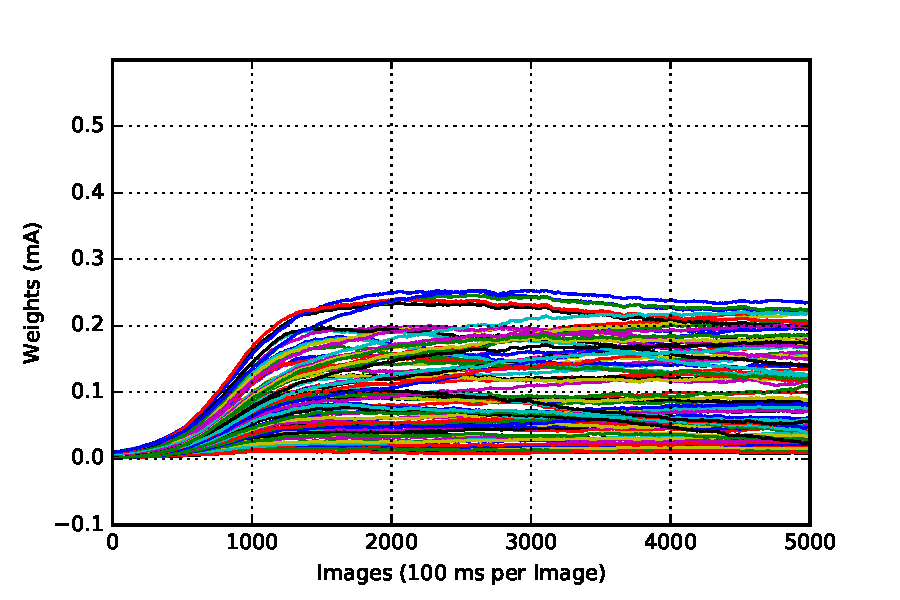
\includegraphics[width=\textwidth]{pics_sdlm/01_exp_SAE_Orig_long/exp2_weights_s.pdf}
		\caption{Weights of Exp2}
	\end{subfigure}
	\begin{subfigure}[t]{0.45\textwidth}
		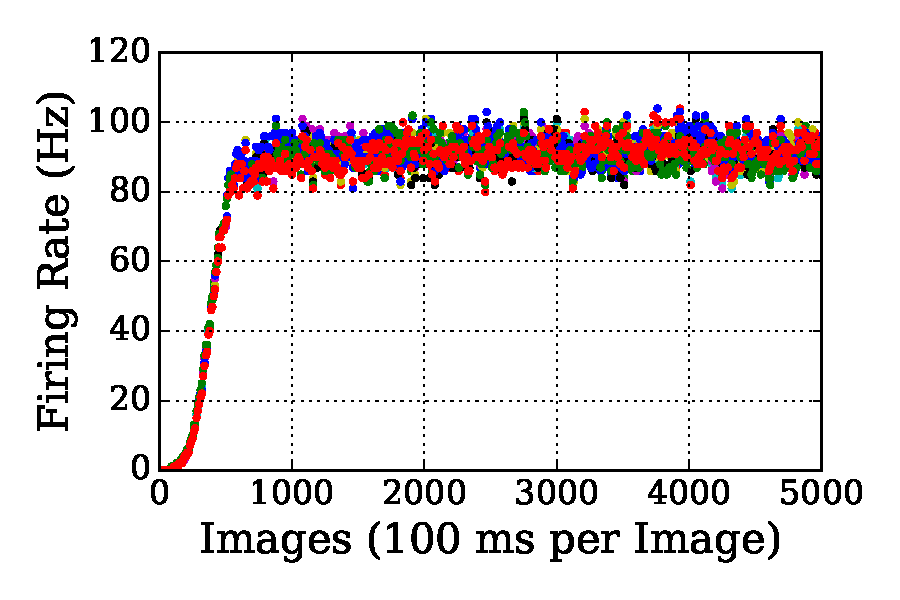
\includegraphics[width=\textwidth]{pics_sdlm/01_exp_SAE_Orig_long/exp1_recon_s.pdf}
		\caption{Reconstruction of visible units in Exp1}
	\end{subfigure}
	\begin{subfigure}[t]{0.45\textwidth}
		\includegraphics[width=\textwidth]{pics_sdlm/01_exp_SAE_Orig_long/exp2_recon_s.pdf}
		\caption{Reconstruction of visible units in Exp2}
	\end{subfigure}\\
	\begin{subfigure}[t]{0.45\textwidth}
		\includegraphics[width=\textwidth]{pics_sdlm/01_exp_SAE_Orig_long/exp1_hid_s.pdf}
		\caption{Output of hidden units in Exp1}
	\end{subfigure}
	\begin{subfigure}[t]{0.45\textwidth}
		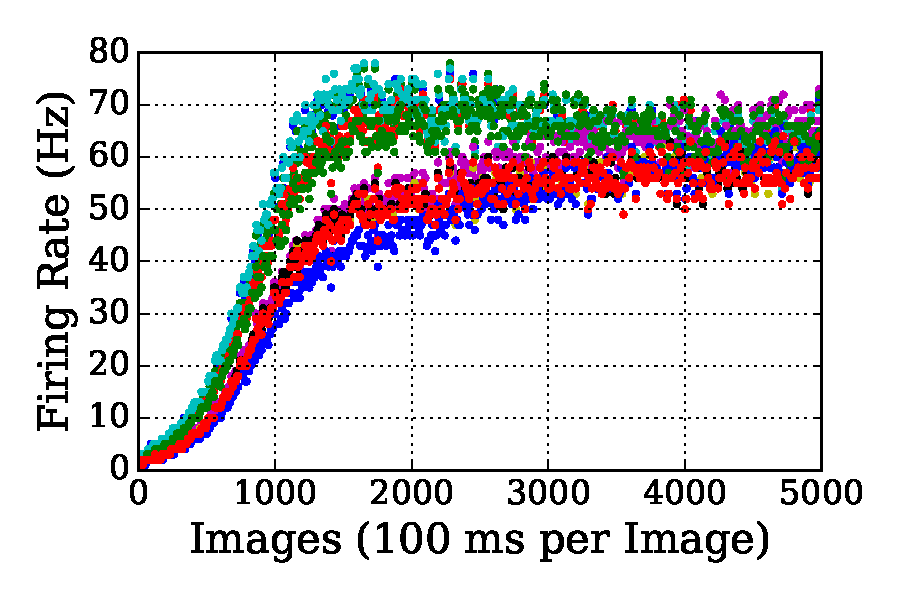
\includegraphics[width=\textwidth]{pics_sdlm/01_exp_SAE_Orig_long/exp2_hid_s.pdf}
		\caption{Output of hidden units in Exp2}
	\end{subfigure}\\
	\begin{subfigure}[t]{0.45\textwidth}
		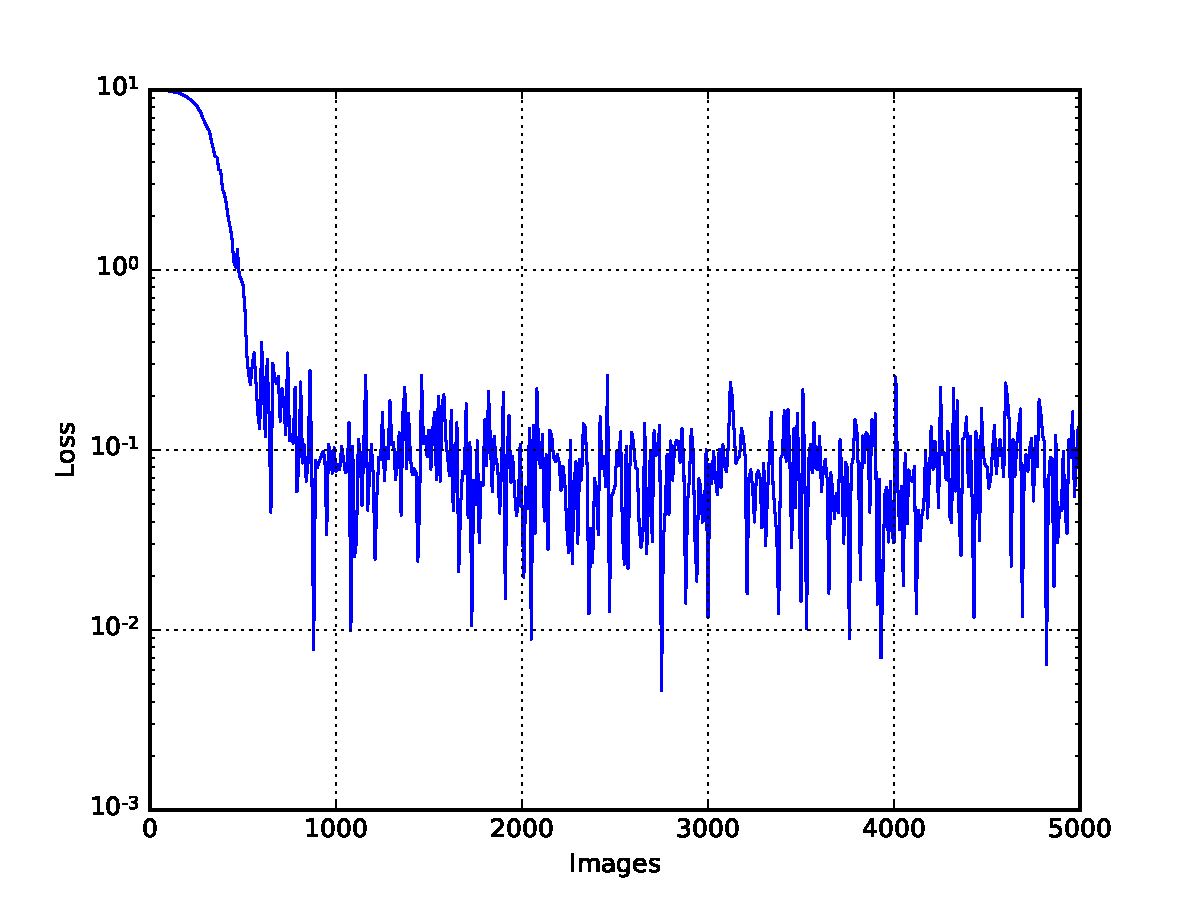
\includegraphics[width=\textwidth]{pics_sdlm/01_exp_SAE_Orig_long/exp1_mse_nons.pdf}
		\caption{Loss of Exp1}
	\end{subfigure}
	\begin{subfigure}[t]{0.45\textwidth}
		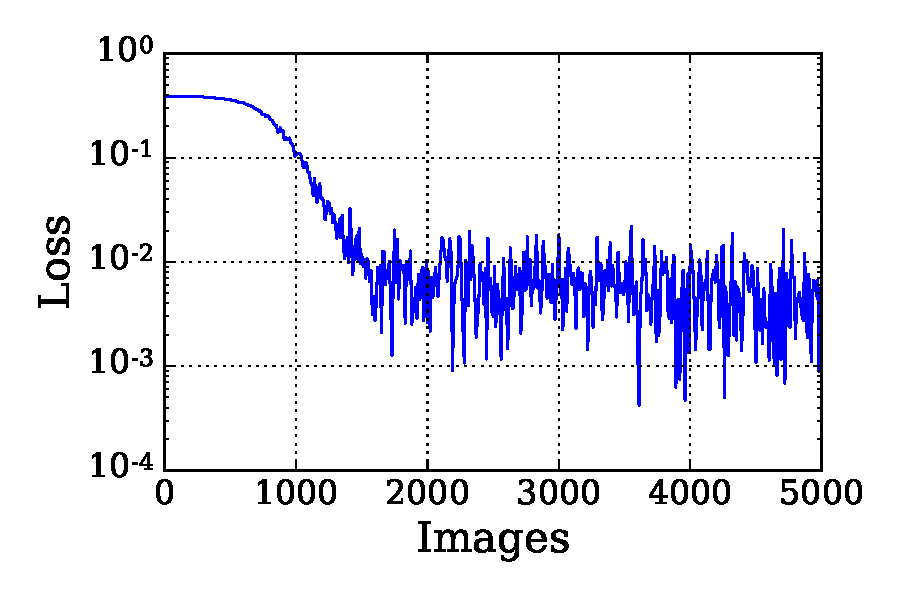
\includegraphics[width=\textwidth]{pics_sdlm/01_exp_SAE_Orig_long/exp2_mse_nons.pdf}
		\caption{Loss of Exp2}
	\end{subfigure}
	\caption{Weights and firing rates of visible and hidden units change during training of the reconstruction tests of spiking AE. 
		Experiments 1) 10 visible units fully connected to 10 hidden units with Poisson spike trains of 100~Hz which lasted 100~ms; 2) same network fed with 10 Poisson spike trains of firing rate ranging from 10~Hz to 100~Hz.}
	\label{fig:sol1_ae}
\end{figure}

\begin{figure}
	\centering
	\begin{subfigure}[t]{0.45\textwidth}
		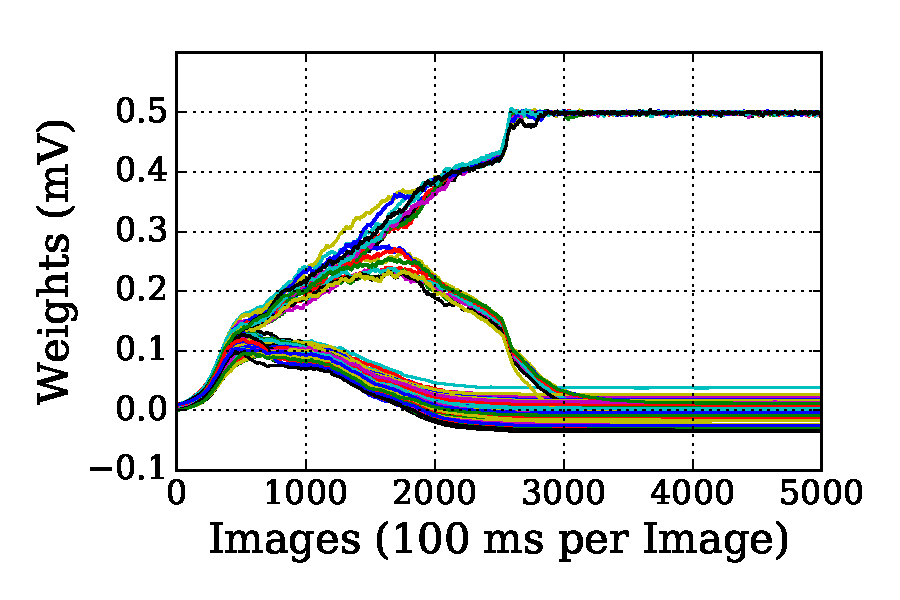
\includegraphics[width=\textwidth]{pics_sdlm/11_exp_SRBM_Orig_long/exp1_weights_s.pdf}
		\caption{Weights of Exp1}
	\end{subfigure}
	\begin{subfigure}[t]{0.45\textwidth}
		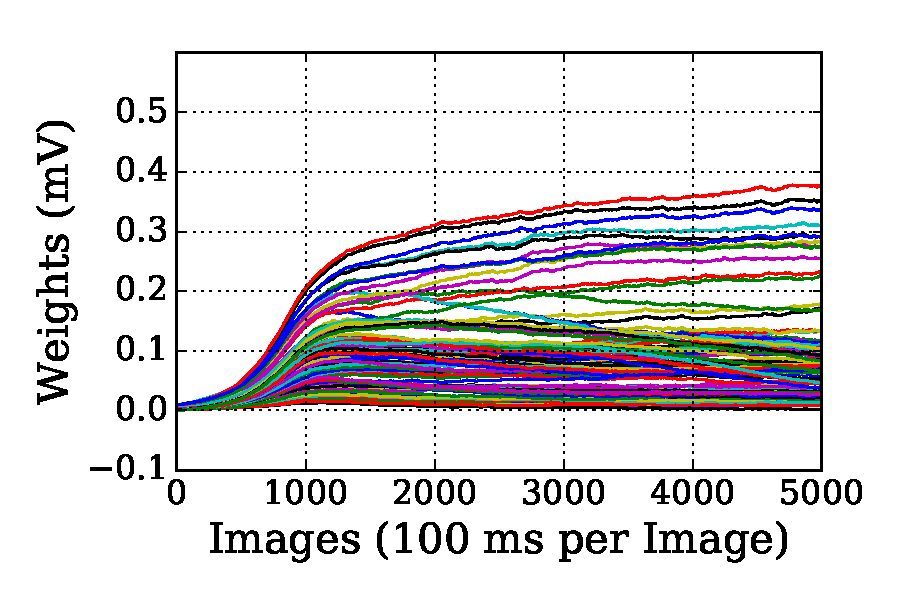
\includegraphics[width=\textwidth]{pics_sdlm/11_exp_SRBM_Orig_long/exp2_weights_s.pdf}
		\caption{Weights of Exp2}
	\end{subfigure}
	\begin{subfigure}[t]{0.45\textwidth}
		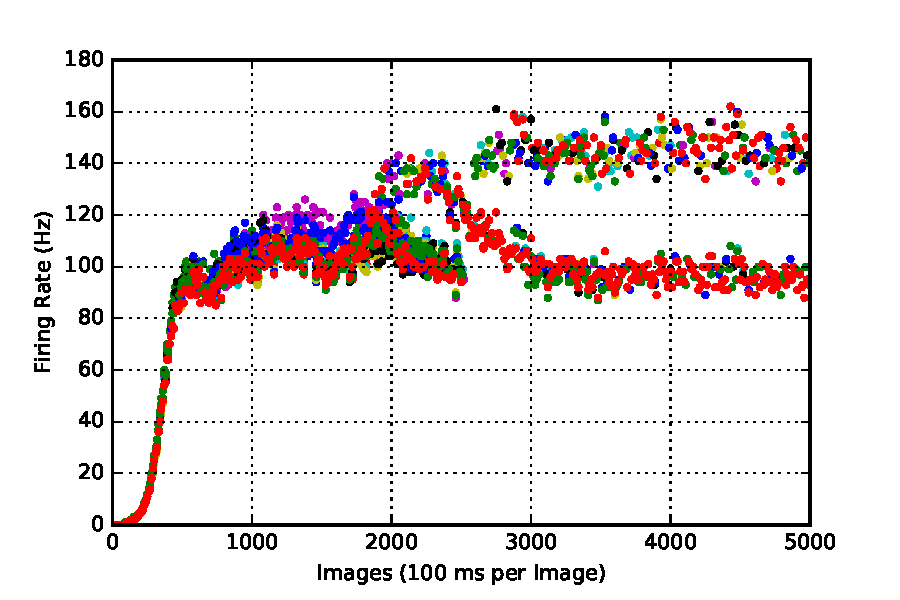
\includegraphics[width=\textwidth]{pics_sdlm/11_exp_SRBM_Orig_long/exp1_recon_s.pdf}
		\caption{Reconstruction of visible units in Exp1}
	\end{subfigure}
	\begin{subfigure}[t]{0.45\textwidth}
		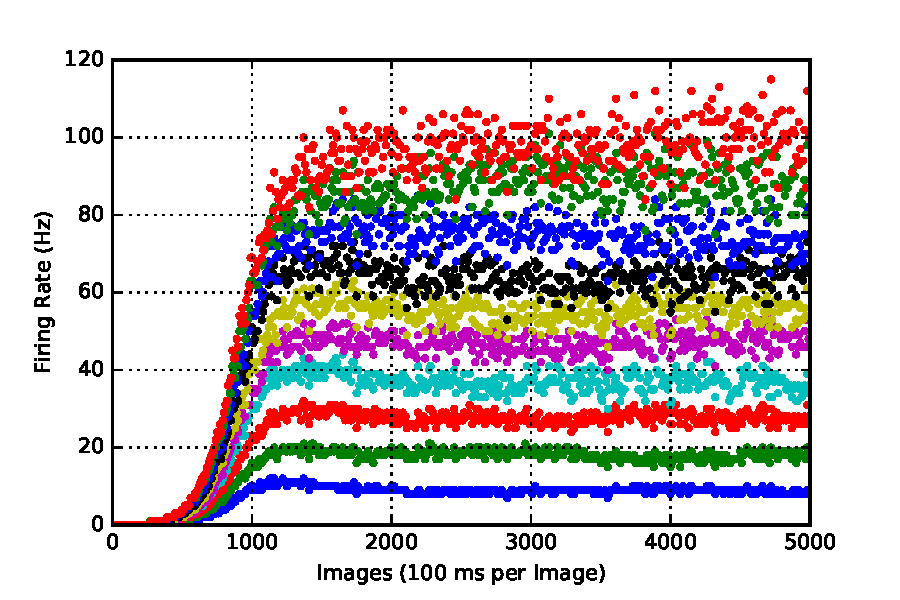
\includegraphics[width=\textwidth]{pics_sdlm/11_exp_SRBM_Orig_long/exp2_recon_s.pdf}
		\caption{Reconstruction of visible units in Exp2}
	\end{subfigure}\\
	\begin{subfigure}[t]{0.45\textwidth}
		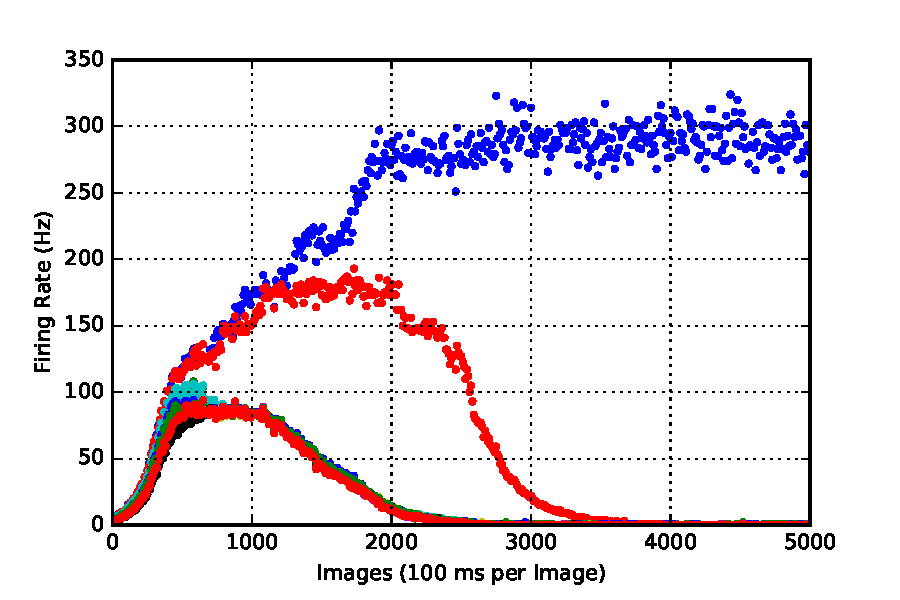
\includegraphics[width=\textwidth]{pics_sdlm/11_exp_SRBM_Orig_long/exp1_hid_s.pdf}
		\caption{Output of hidden units in Exp1}
	\end{subfigure}
	\begin{subfigure}[t]{0.45\textwidth}
		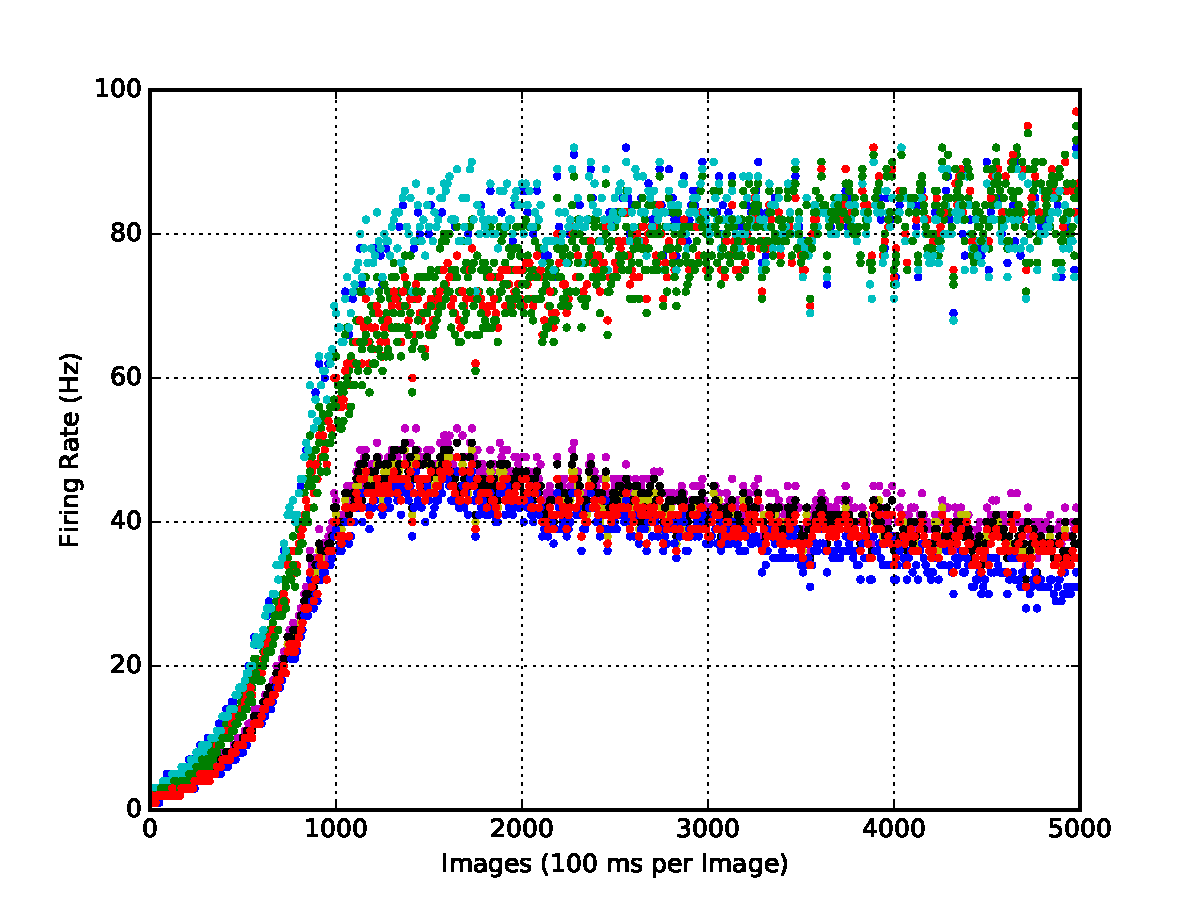
\includegraphics[width=\textwidth]{pics_sdlm/11_exp_SRBM_Orig_long/exp2_hid_s.pdf}
		\caption{Output of hidden units in Exp2}
	\end{subfigure}\\
	\begin{subfigure}[t]{0.45\textwidth}
		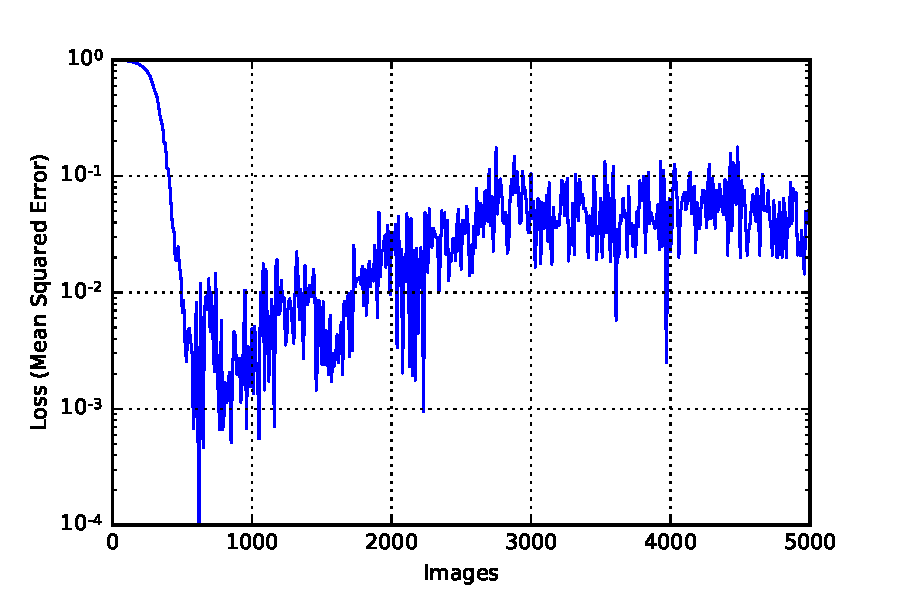
\includegraphics[width=\textwidth]{pics_sdlm/11_exp_SRBM_Orig_long/exp1_mse_nons.pdf}
		\caption{Loss of Exp1}
	\end{subfigure}
	\begin{subfigure}[t]{0.45\textwidth}
		\includegraphics[width=\textwidth]{pics_sdlm/11_exp_SRBM_Orig_long/exp2_mse_nons.pdf}
		\caption{Loss of Exp2}
	\end{subfigure}
	\caption{Weights and firing rates of visible and hidden units change during training of the reconstruction tests of spiking RBM. 
		Experiments 1) 10 visible units fully connected to 10 hidden units with Poisson spike trains of 100~Hz which lasted 100~ms; 2) same network fed with 10 Poisson spike trains of firing rate ranging from 10~Hz to 100~Hz.}
	\label{fig:sol1_rbm}
\end{figure}

\begin{figure}
	\centering
	\begin{subfigure}[t]{0.45\textwidth}
		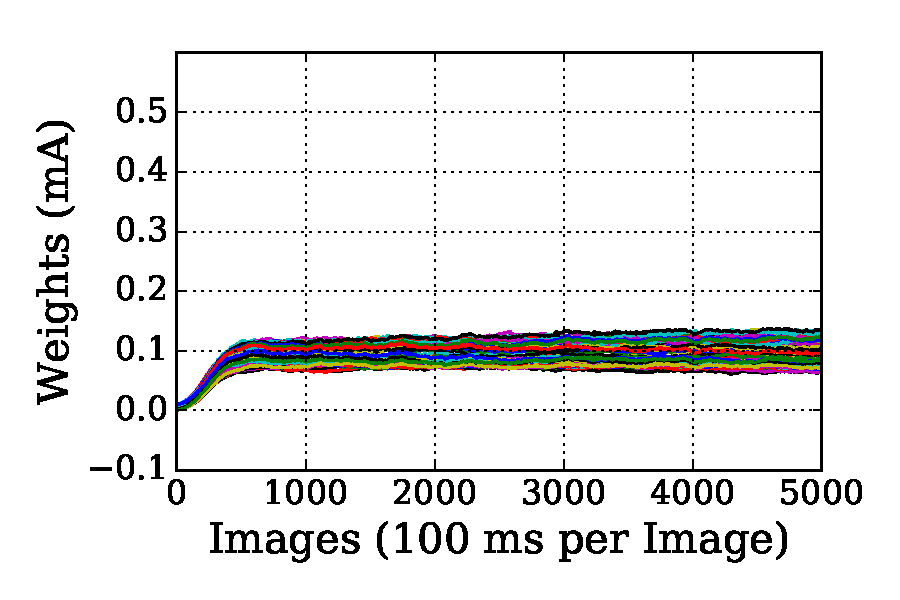
\includegraphics[width=\textwidth]{pics_sdlm/03_exp_SAE_noise_long/exp1_weights_s.pdf}
		\caption{Weights of Exp1}
	\end{subfigure}
	\begin{subfigure}[t]{0.45\textwidth}
		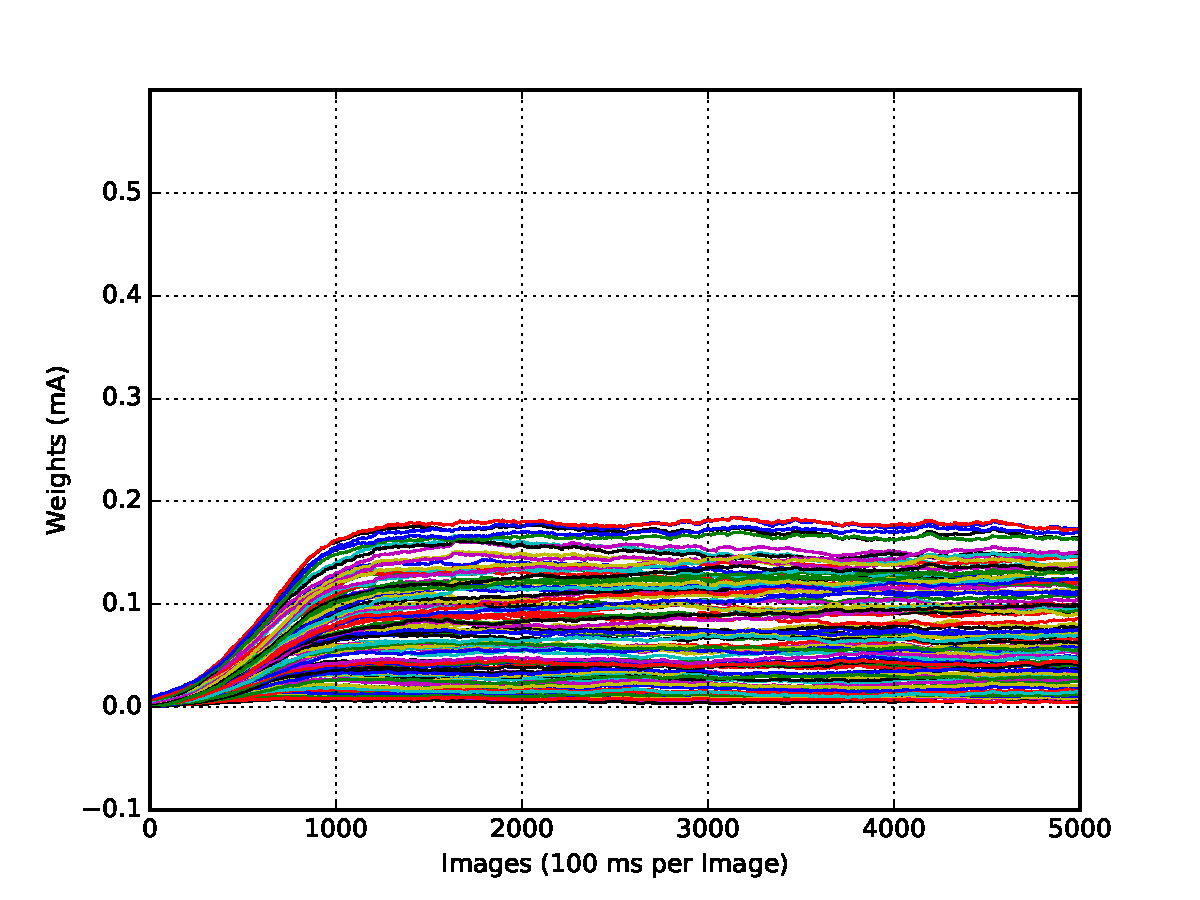
\includegraphics[width=\textwidth]{pics_sdlm/03_exp_SAE_noise_long/exp2_weights_s.pdf}
		\caption{Weights of Exp2}
	\end{subfigure}
	\begin{subfigure}[t]{0.45\textwidth}
		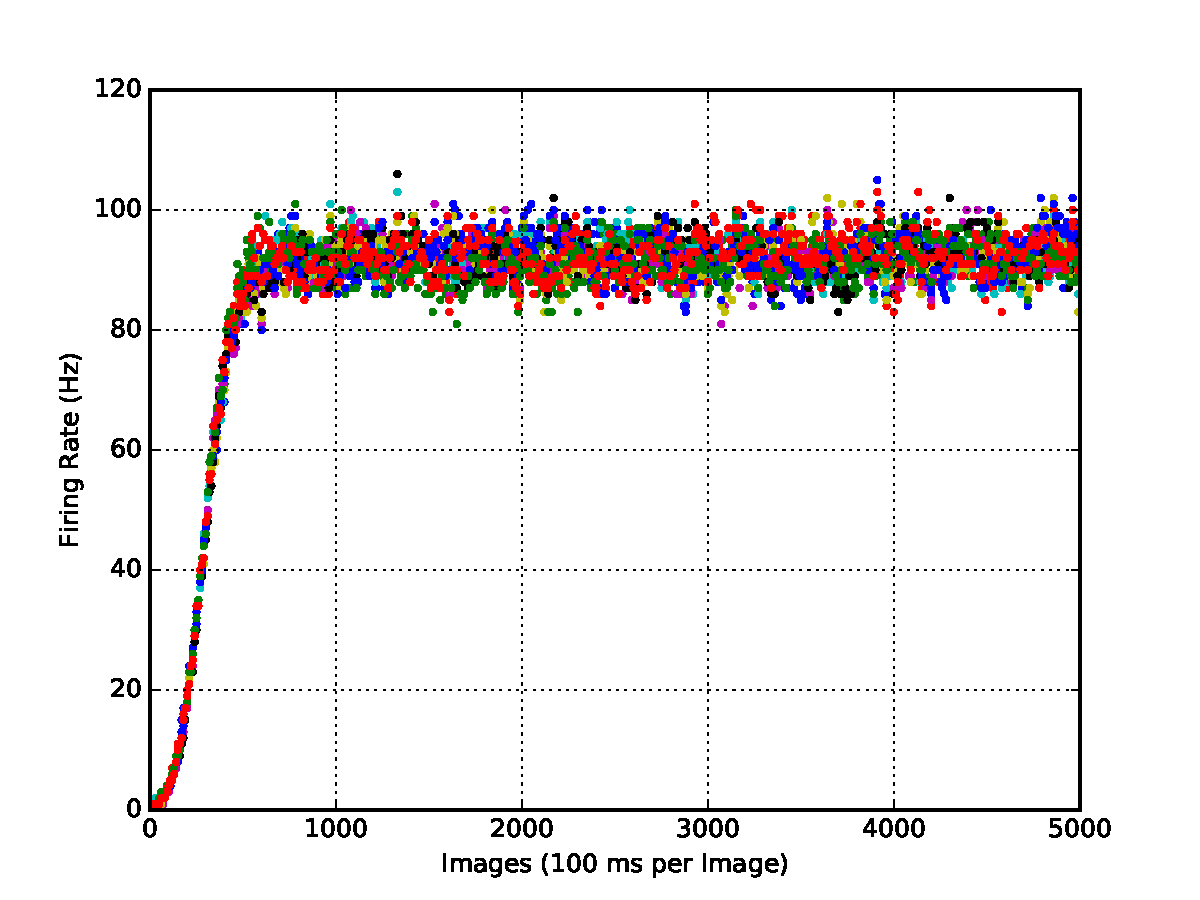
\includegraphics[width=\textwidth]{pics_sdlm/03_exp_SAE_noise_long/exp1_recon_s.pdf}
		\caption{Reconstruction of visible units in Exp1}
	\end{subfigure}
	\begin{subfigure}[t]{0.45\textwidth}
		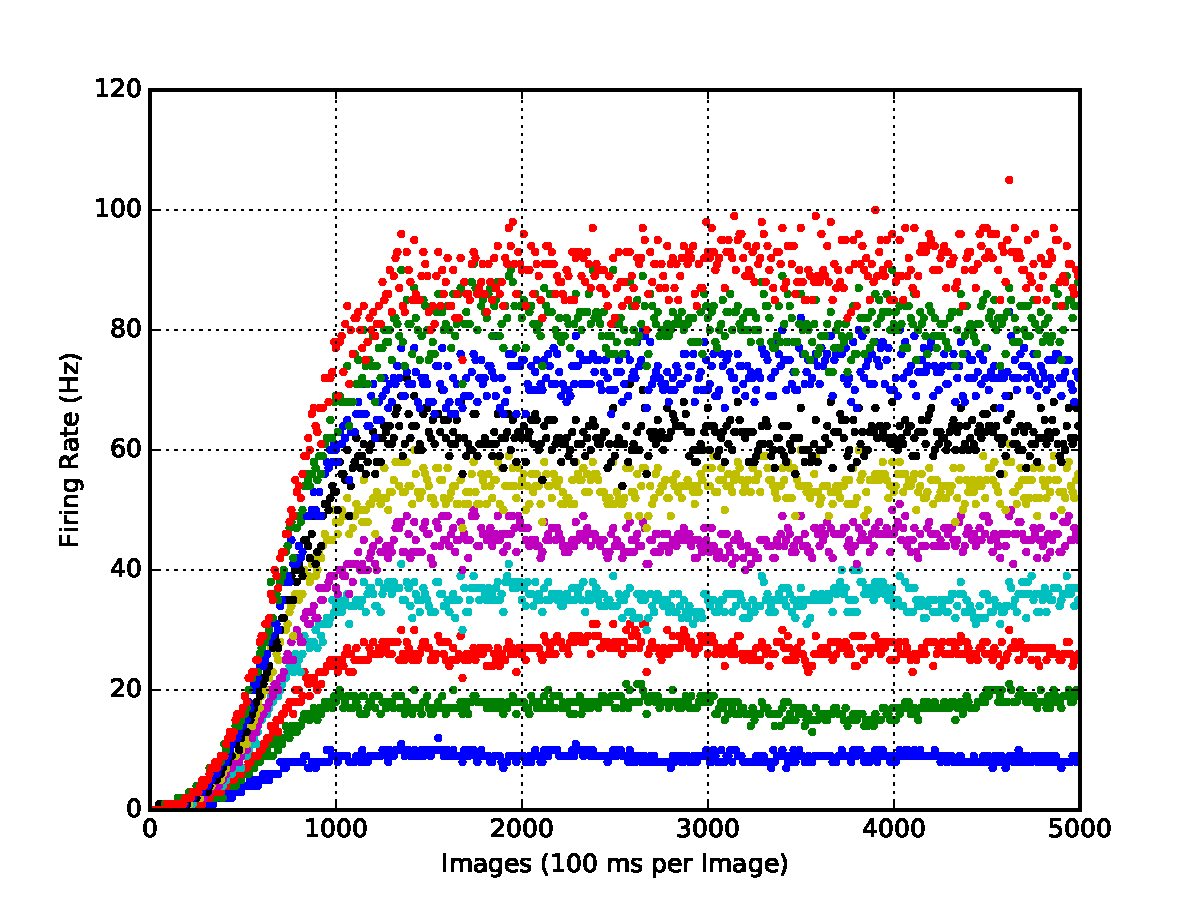
\includegraphics[width=\textwidth]{pics_sdlm/03_exp_SAE_noise_long/exp2_recon_s.pdf}
		\caption{Reconstruction of visible units in Exp2}
	\end{subfigure}\\
	\begin{subfigure}[t]{0.45\textwidth}
		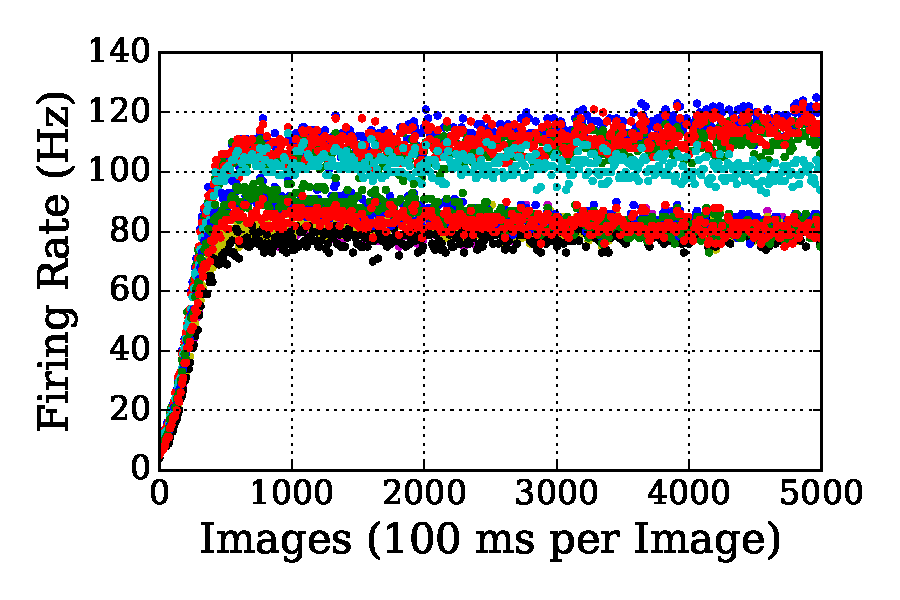
\includegraphics[width=\textwidth]{pics_sdlm/03_exp_SAE_noise_long/exp1_hid_s.pdf}
		\caption{Output of hidden units in Exp1}
	\end{subfigure}
	\begin{subfigure}[t]{0.45\textwidth}
		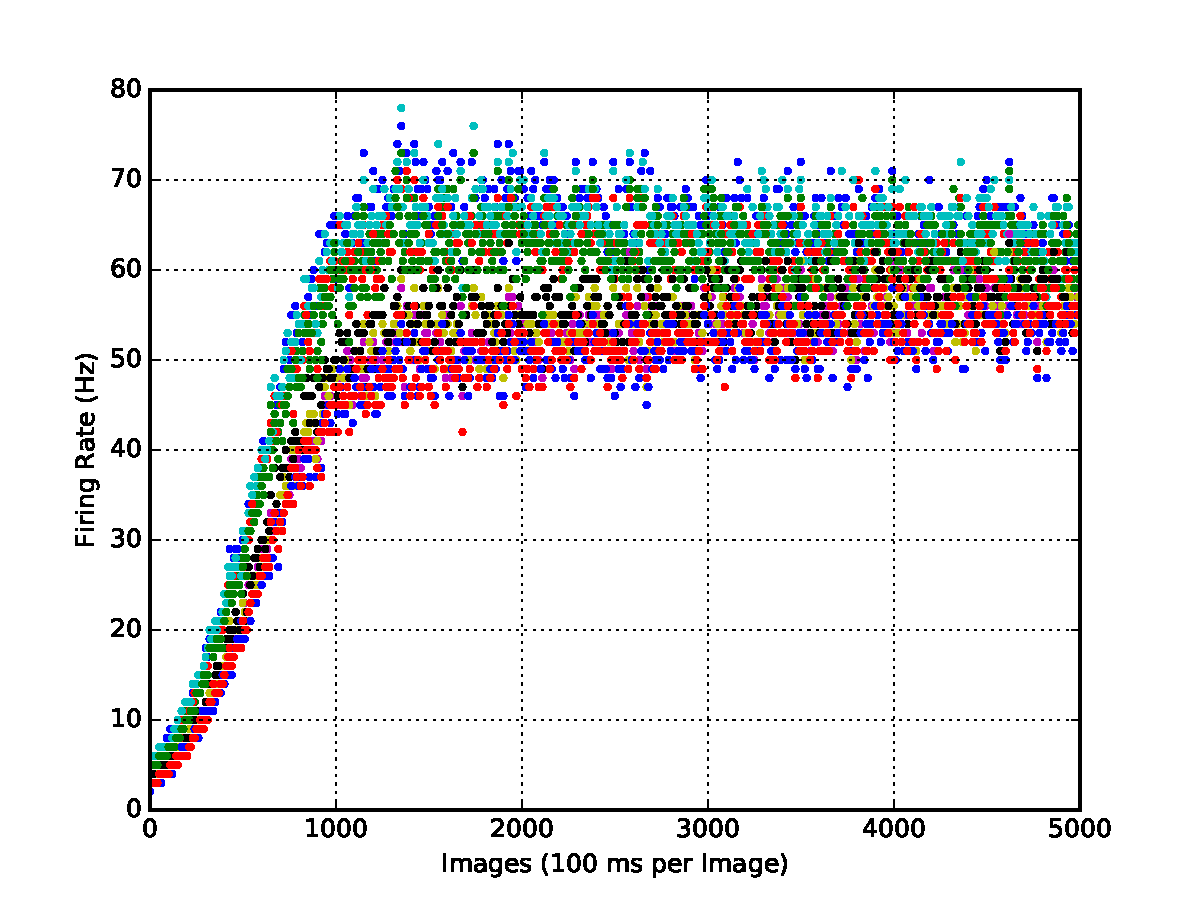
\includegraphics[width=\textwidth]{pics_sdlm/03_exp_SAE_noise_long/exp2_hid_s.pdf}
		\caption{Output of hidden units in Exp2}
	\end{subfigure}\\
	\begin{subfigure}[t]{0.45\textwidth}
		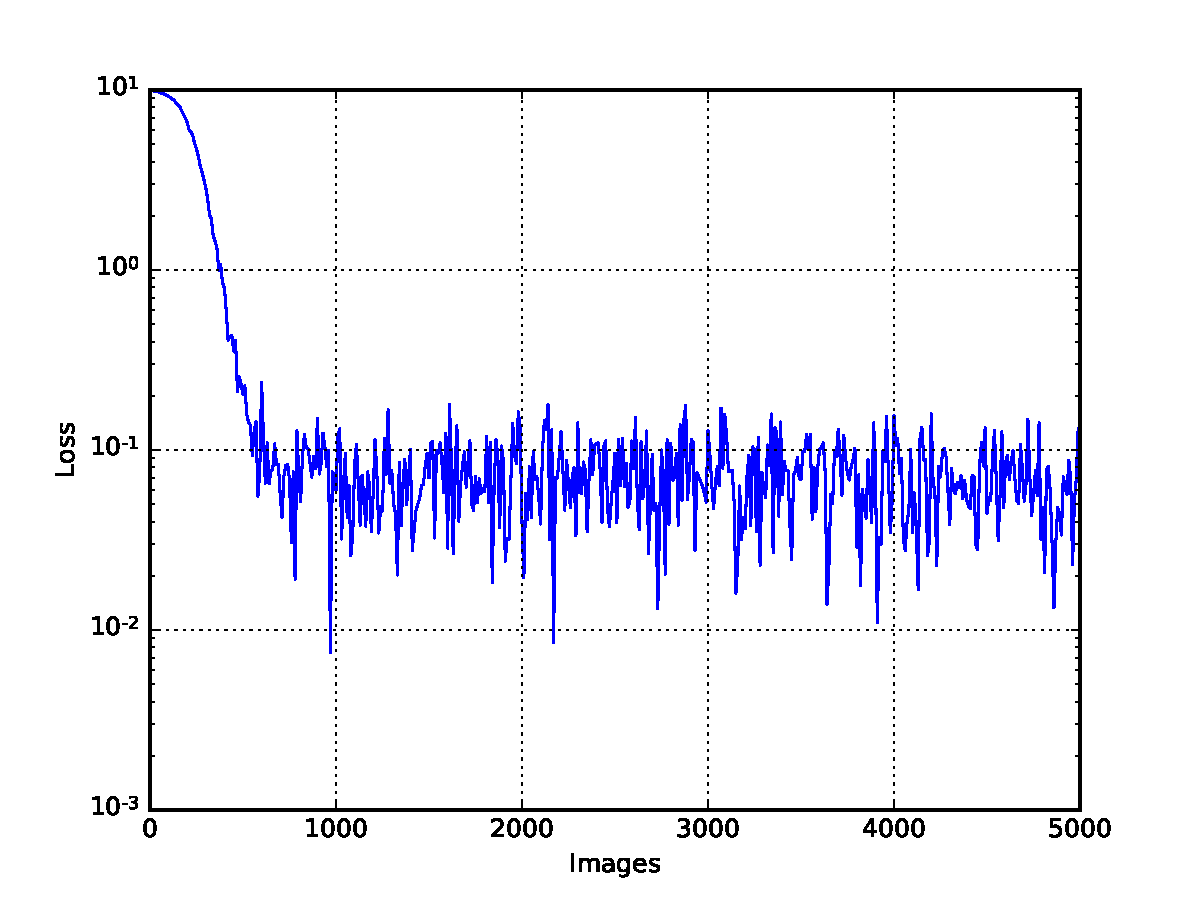
\includegraphics[width=\textwidth]{pics_sdlm/03_exp_SAE_noise_long/exp1_mse_nons.pdf}
		\caption{Loss of Exp1}
	\end{subfigure}
	\begin{subfigure}[t]{0.45\textwidth}
		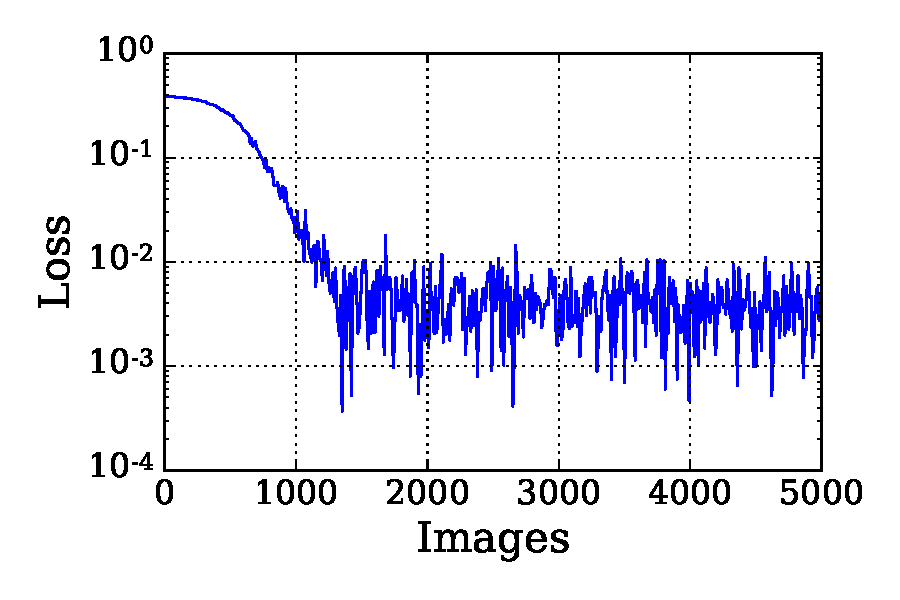
\includegraphics[width=\textwidth]{pics_sdlm/03_exp_SAE_noise_long/exp2_mse_nons.pdf}
		\caption{Loss of Exp2}
	\end{subfigure}
	\caption{Weights and firing rates of visible and hidden units change during training of the reconstruction tests of spiking AE. 
		Experiments 1) 10 visible units fully connected to 10 hidden units with Poisson spike trains of 100~Hz which lasted 100~ms; 2) same network fed with 10 Poisson spike trains of firing rate ranging from 10~Hz to 100~Hz.}
	\label{fig:sol2_ae}
\end{figure}

\begin{figure}
	\centering
	\begin{subfigure}[t]{0.45\textwidth}
		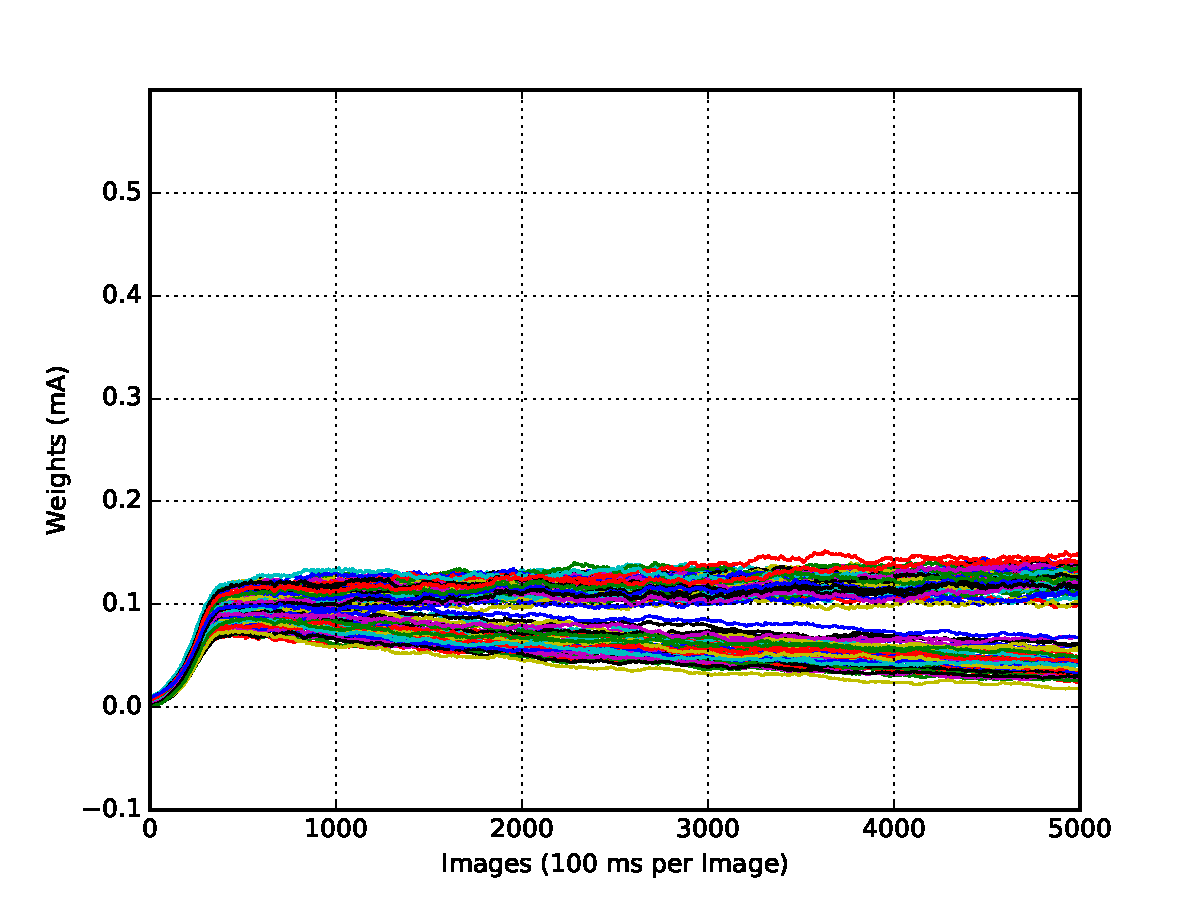
\includegraphics[width=\textwidth]{pics_sdlm/13_exp_SRBM_noise_long/exp1_weights_s.pdf}
		\caption{Weights of Exp1}
	\end{subfigure}
	\begin{subfigure}[t]{0.45\textwidth}
		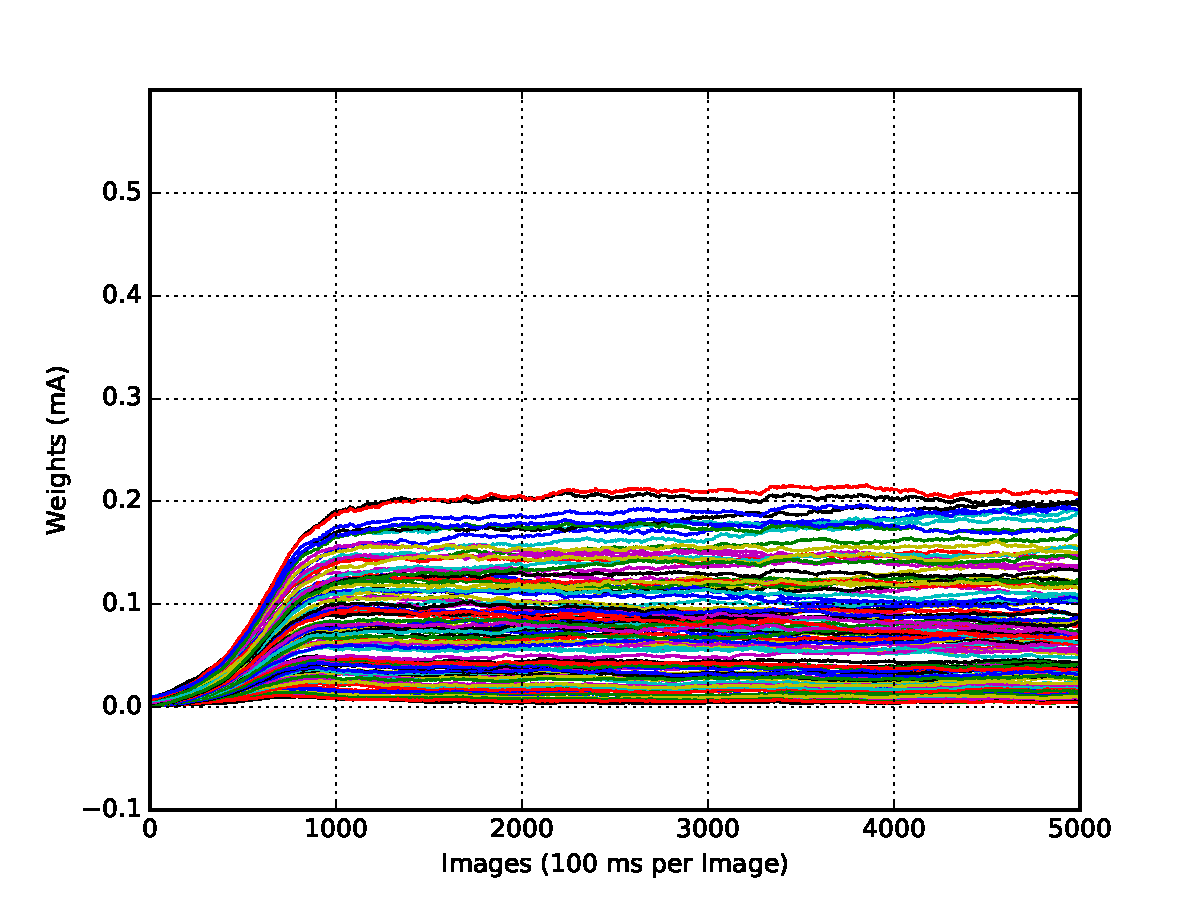
\includegraphics[width=\textwidth]{pics_sdlm/13_exp_SRBM_noise_long/exp2_weights_s.pdf}
		\caption{Weights of Exp2}
	\end{subfigure}
	\begin{subfigure}[t]{0.45\textwidth}
		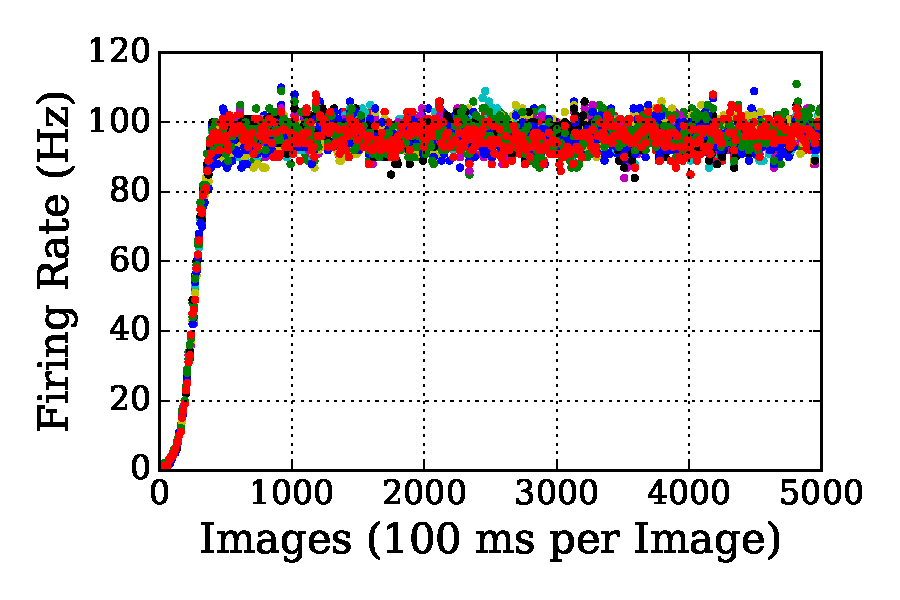
\includegraphics[width=\textwidth]{pics_sdlm/13_exp_SRBM_noise_long/exp1_recon_s.pdf}
		\caption{Reconstruction of visible units in Exp1}
	\end{subfigure}
	\begin{subfigure}[t]{0.45\textwidth}
		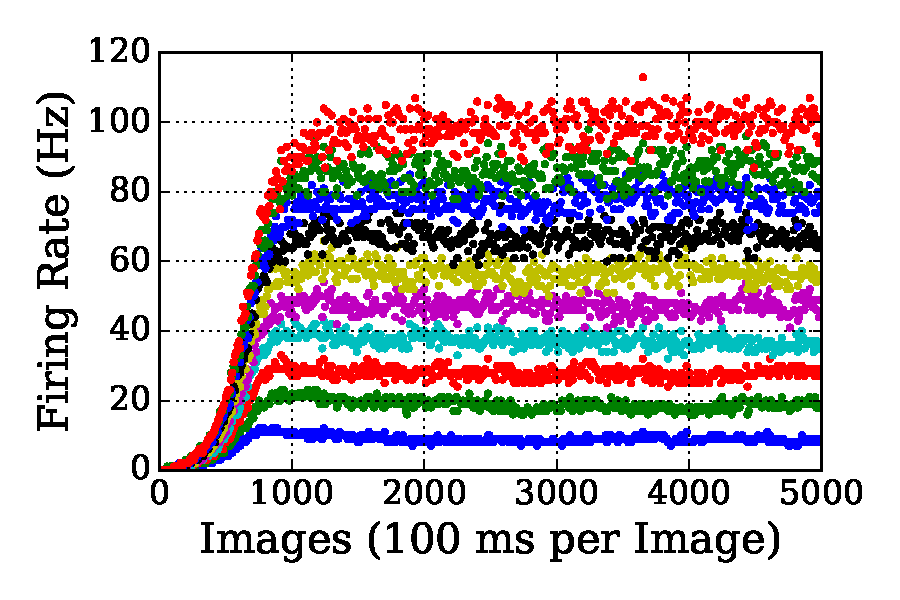
\includegraphics[width=\textwidth]{pics_sdlm/13_exp_SRBM_noise_long/exp2_recon_s.pdf}
		\caption{Reconstruction of visible units in Exp2}
	\end{subfigure}\\
	\begin{subfigure}[t]{0.45\textwidth}
		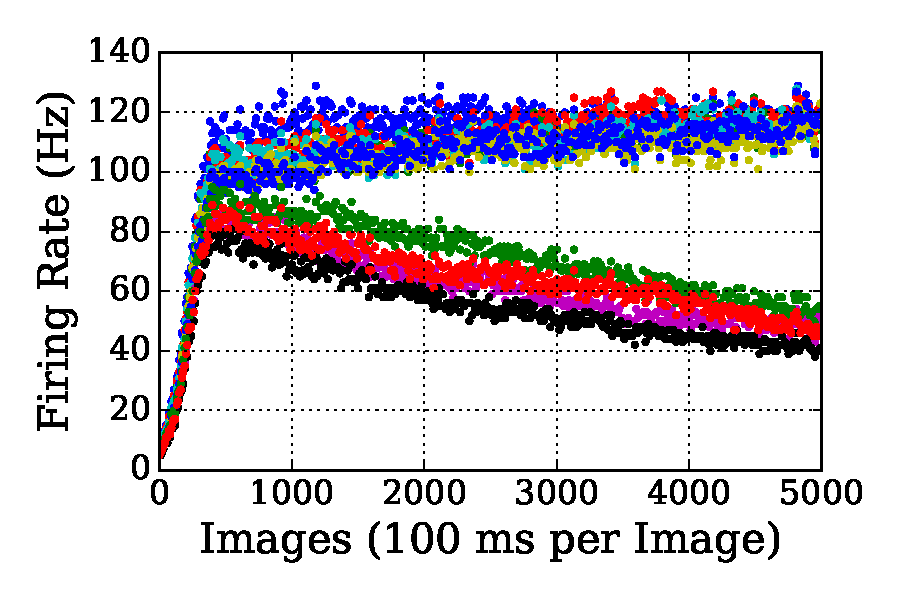
\includegraphics[width=\textwidth]{pics_sdlm/13_exp_SRBM_noise_long/exp1_hid_s.pdf}
		\caption{Output of hidden units in Exp1}
	\end{subfigure}
	\begin{subfigure}[t]{0.45\textwidth}
		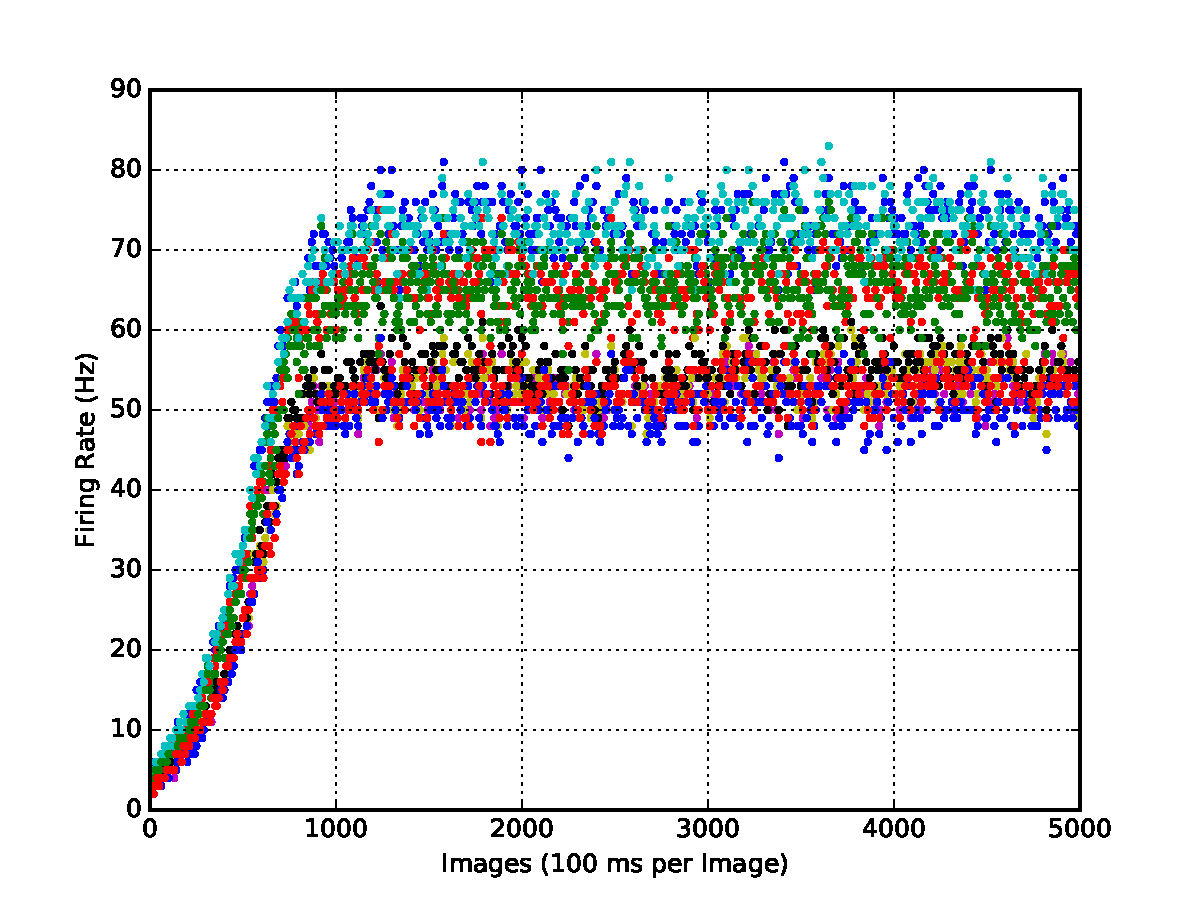
\includegraphics[width=\textwidth]{pics_sdlm/13_exp_SRBM_noise_long/exp2_hid_s.pdf}
		\caption{Output of hidden units in Exp2}
	\end{subfigure}\\
	\begin{subfigure}[t]{0.45\textwidth}
		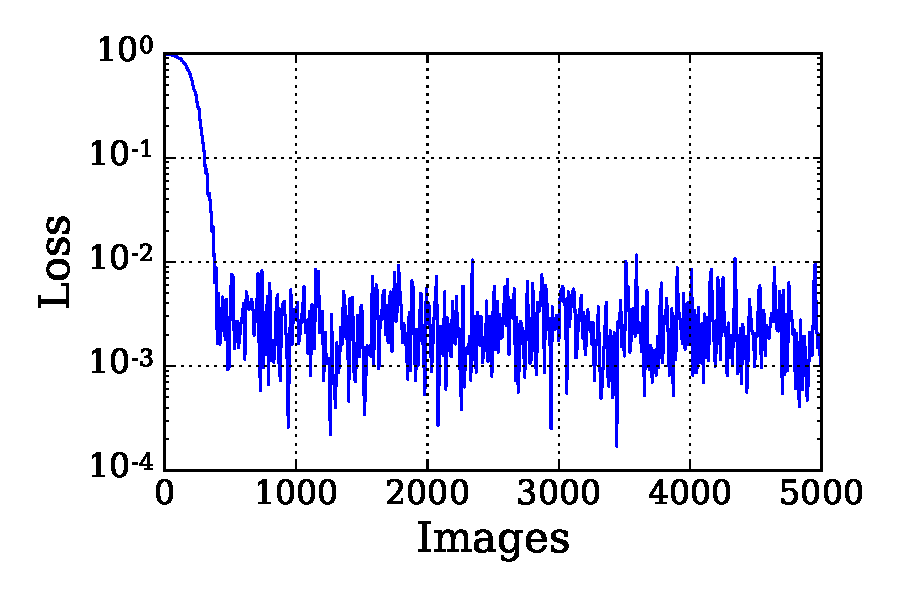
\includegraphics[width=\textwidth]{pics_sdlm/13_exp_SRBM_noise_long/exp1_mse_nons.pdf}
		\caption{Loss of Exp1}
	\end{subfigure}
	\begin{subfigure}[t]{0.45\textwidth}
		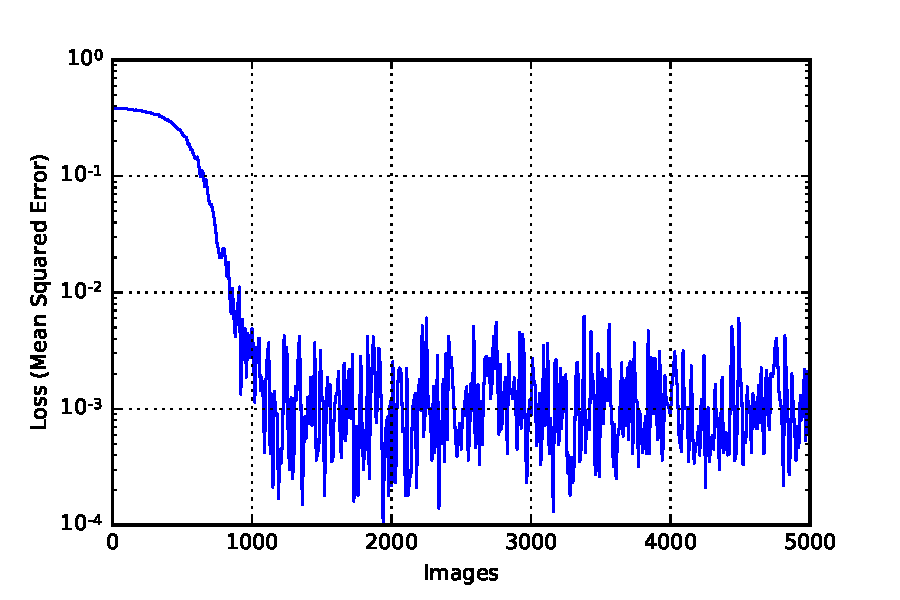
\includegraphics[width=\textwidth]{pics_sdlm/13_exp_SRBM_noise_long/exp2_mse_nons.pdf}
		\caption{Loss of Exp2}
	\end{subfigure}
	\caption{Weights and firing rates of visible and hidden units change during training of the reconstruction tests of spiking RBM. 
		Experiments 1) 10 visible units fully connected to 10 hidden units with Poisson spike trains of 100~Hz which lasted 100~ms; 2) same network fed with 10 Poisson spike trains of firing rate ranging from 10~Hz to 100~Hz.}
	\label{fig:sol2_rbm}
\end{figure}

\begin{figure}
	\centering
	\begin{subfigure}[t]{0.45\textwidth}
		\includegraphics[width=\textwidth]{pics_sdlm/05_exp_SAE_teach_long/exp1_weights_s.pdf}
		\caption{Weights of Exp1}
	\end{subfigure}
	\begin{subfigure}[t]{0.45\textwidth}
		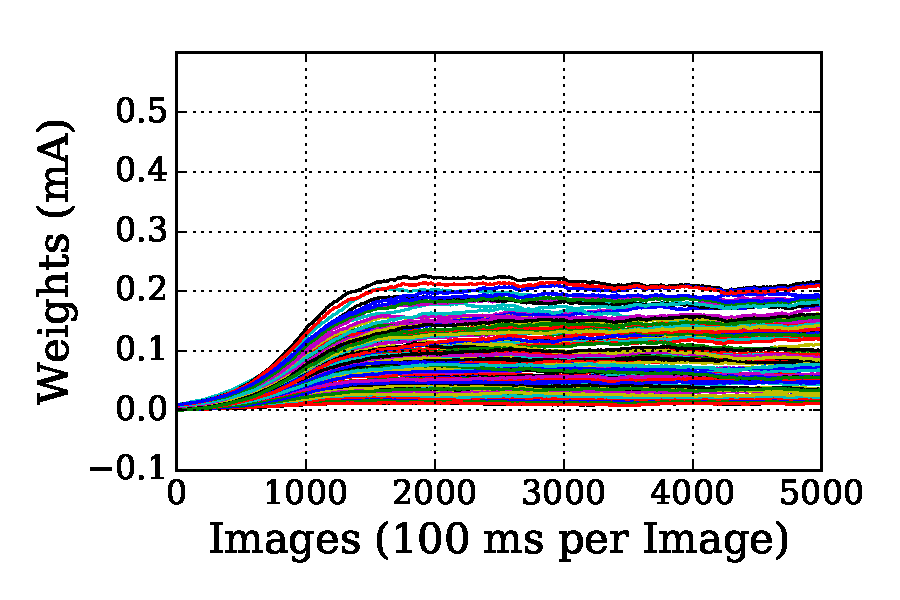
\includegraphics[width=\textwidth]{pics_sdlm/05_exp_SAE_teach_long/exp2_weights_s.pdf}
		\caption{Weights of Exp2}
	\end{subfigure}
	\begin{subfigure}[t]{0.45\textwidth}
		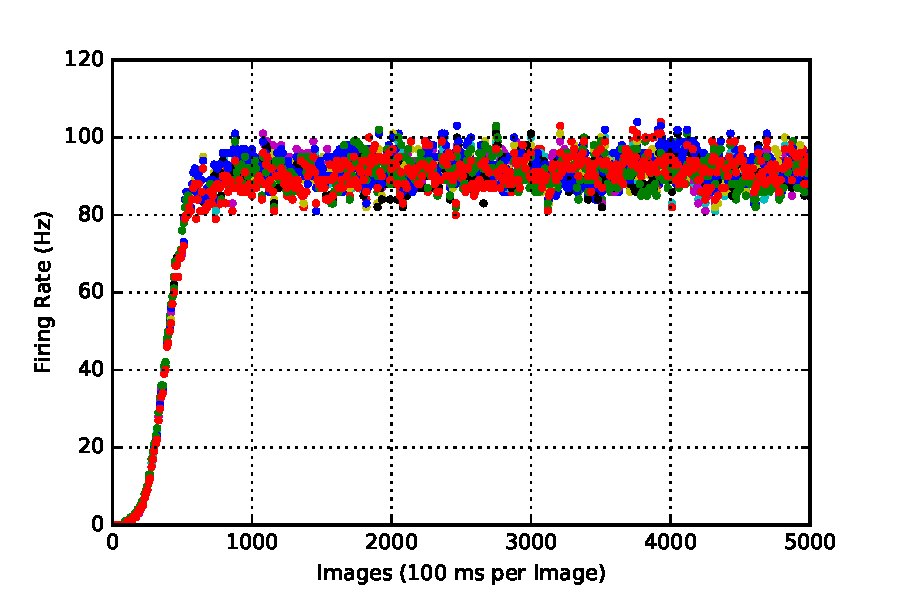
\includegraphics[width=\textwidth]{pics_sdlm/05_exp_SAE_teach_long/exp1_recon_s.pdf}
		\caption{Reconstruction of visible units in Exp1}
	\end{subfigure}
	\begin{subfigure}[t]{0.45\textwidth}
		\includegraphics[width=\textwidth]{pics_sdlm/05_exp_SAE_teach_long/exp2_recon_s.pdf}
		\caption{Reconstruction of visible units in Exp2}
	\end{subfigure}\\
	\begin{subfigure}[t]{0.45\textwidth}
		\includegraphics[width=\textwidth]{pics_sdlm/05_exp_SAE_teach_long/exp1_hid_s.pdf}
		\caption{Output of hidden units in Exp1}
	\end{subfigure}
	\begin{subfigure}[t]{0.45\textwidth}
		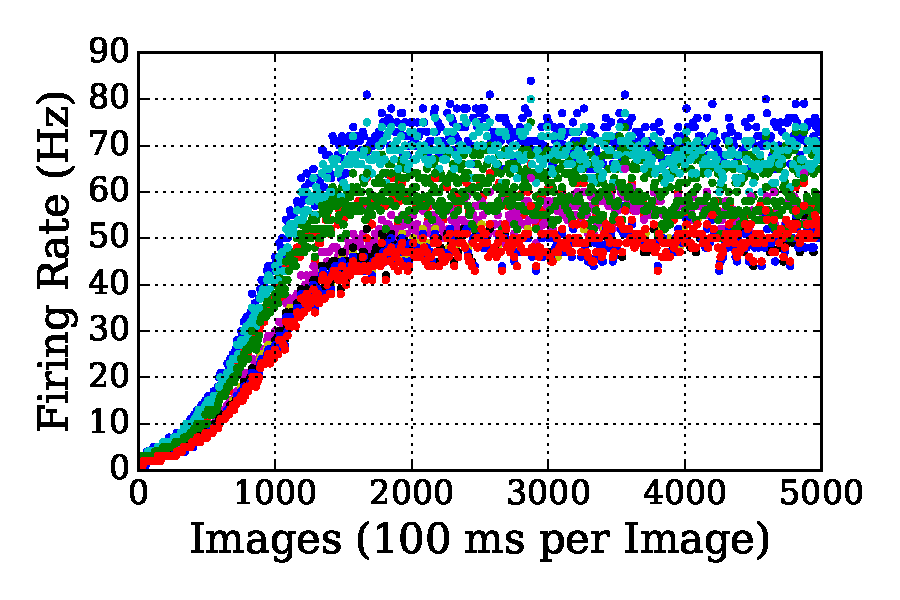
\includegraphics[width=\textwidth]{pics_sdlm/05_exp_SAE_teach_long/exp2_hid_s.pdf}
		\caption{Output of hidden units in Exp2}
	\end{subfigure}\\
	\begin{subfigure}[t]{0.45\textwidth}
		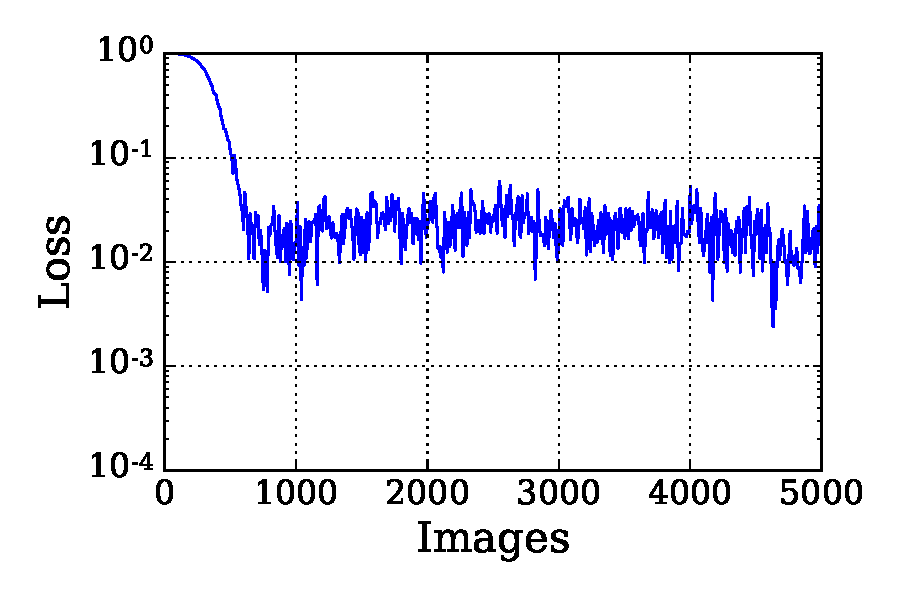
\includegraphics[width=\textwidth]{pics_sdlm/05_exp_SAE_teach_long/exp1_mse_nons.pdf}
		\caption{Loss of Exp1}
	\end{subfigure}
	\begin{subfigure}[t]{0.45\textwidth}
		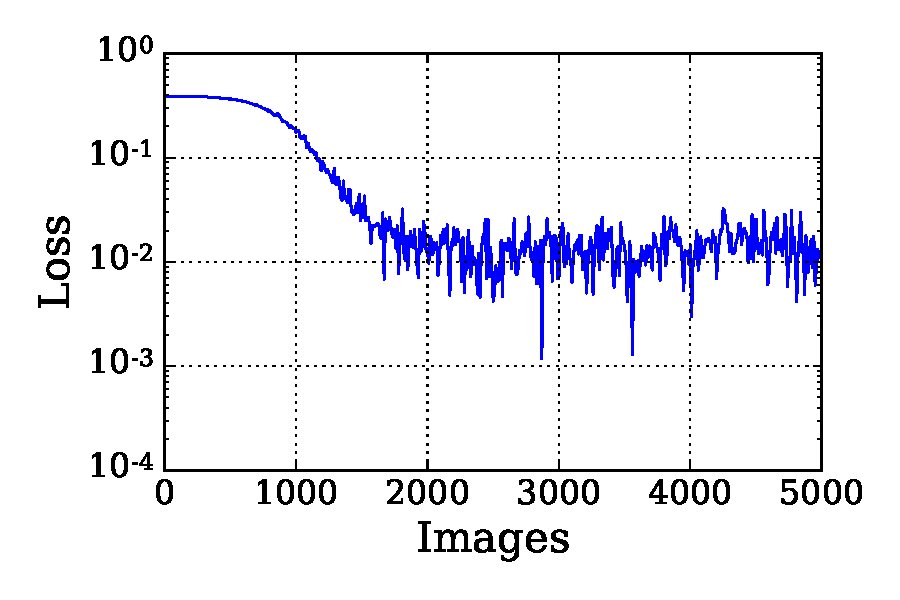
\includegraphics[width=\textwidth]{pics_sdlm/05_exp_SAE_teach_long/exp2_mse_nons.pdf}
		\caption{Loss of Exp2}
	\end{subfigure}
	\caption{Weights and firing rates of visible and hidden units change during training of the reconstruction tests of spiking AE. 
		Experiments 1) 10 visible units fully connected to 10 hidden units with Poisson spike trains of 100~Hz which lasted 100~ms; 2) same network fed with 10 Poisson spike trains of firing rate ranging from 10~Hz to 100~Hz.}
	\label{fig:sol3_ae}
\end{figure}

\begin{figure}
	\centering
	\begin{subfigure}[t]{0.45\textwidth}
		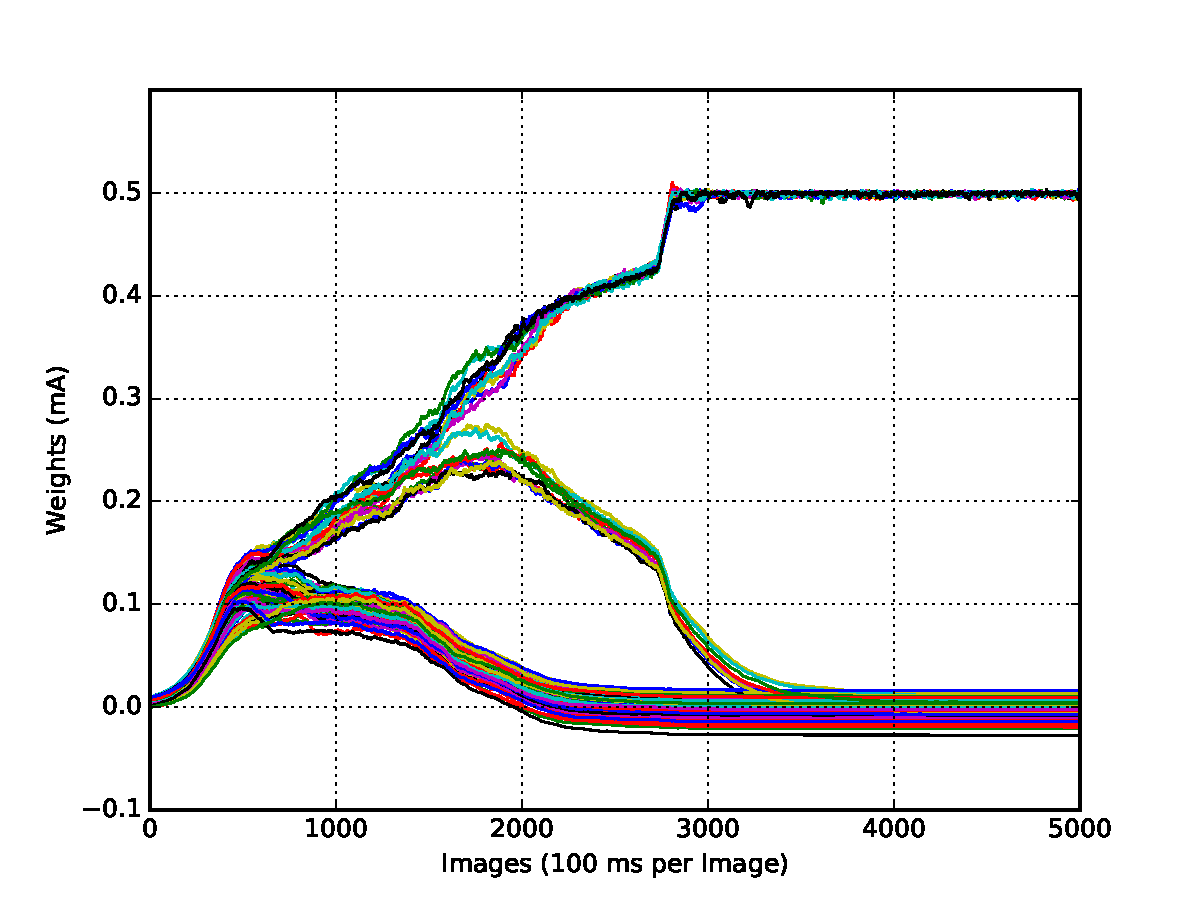
\includegraphics[width=\textwidth]{pics_sdlm/15_exp_SRBM_teach_long/exp1_weights_s.pdf}
		\caption{Weights of Exp1}
	\end{subfigure}
	\begin{subfigure}[t]{0.45\textwidth}
		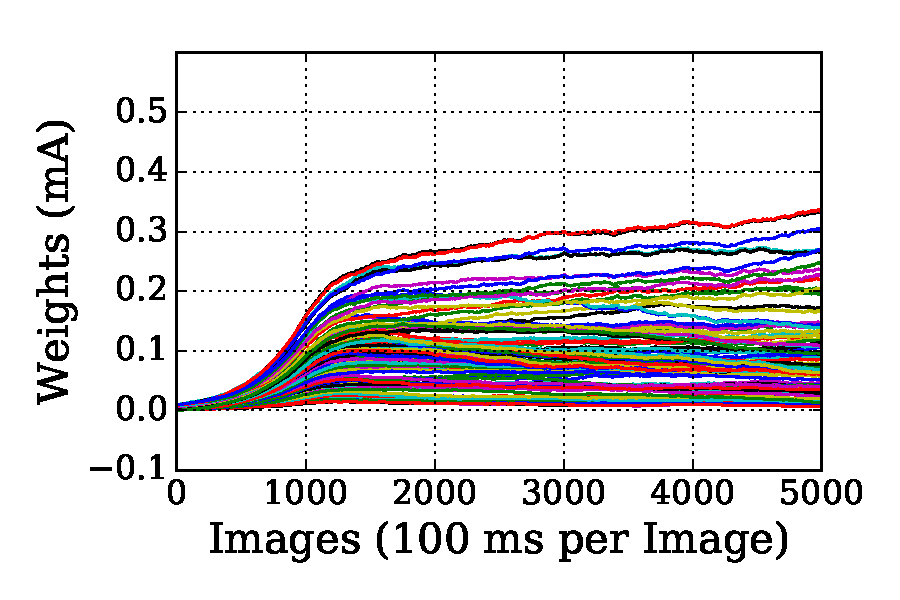
\includegraphics[width=\textwidth]{pics_sdlm/15_exp_SRBM_teach_long/exp2_weights_s.pdf}
		\caption{Weights of Exp2}
	\end{subfigure}
	\begin{subfigure}[t]{0.45\textwidth}
		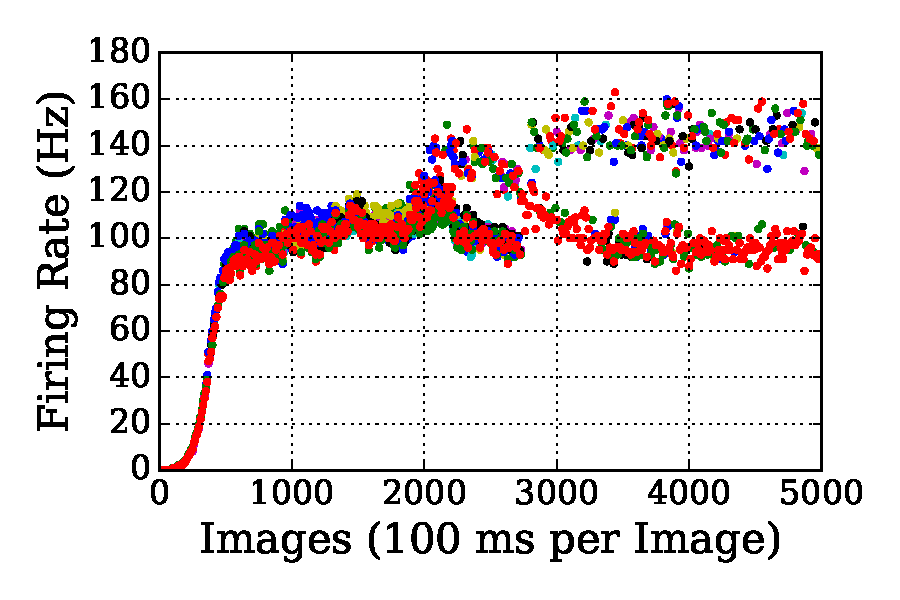
\includegraphics[width=\textwidth]{pics_sdlm/15_exp_SRBM_teach_long/exp1_recon_s.pdf}
		\caption{Reconstruction of visible units in Exp1}
	\end{subfigure}
	\begin{subfigure}[t]{0.45\textwidth}
		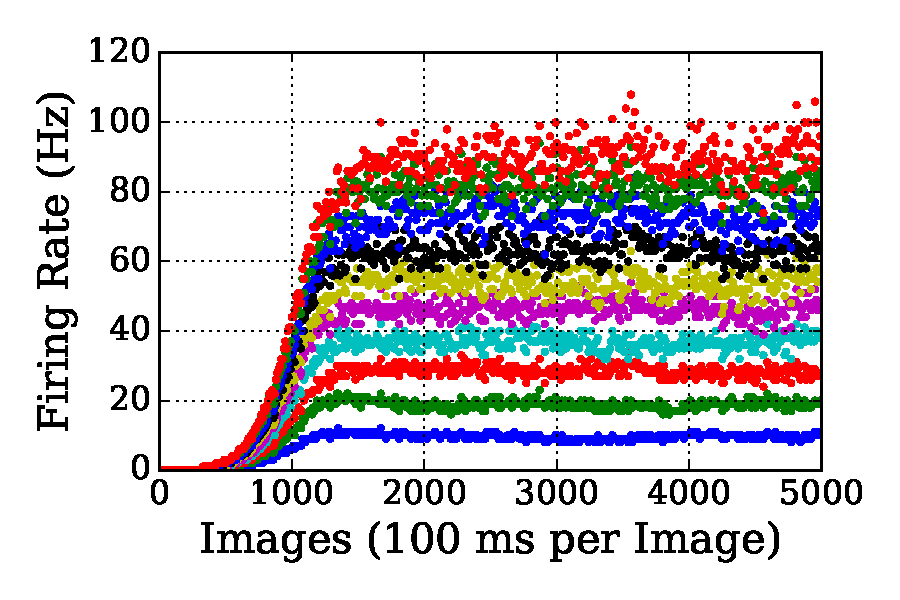
\includegraphics[width=\textwidth]{pics_sdlm/15_exp_SRBM_teach_long/exp2_recon_s.pdf}
		\caption{Reconstruction of visible units in Exp2}
	\end{subfigure}\\
	\begin{subfigure}[t]{0.45\textwidth}
		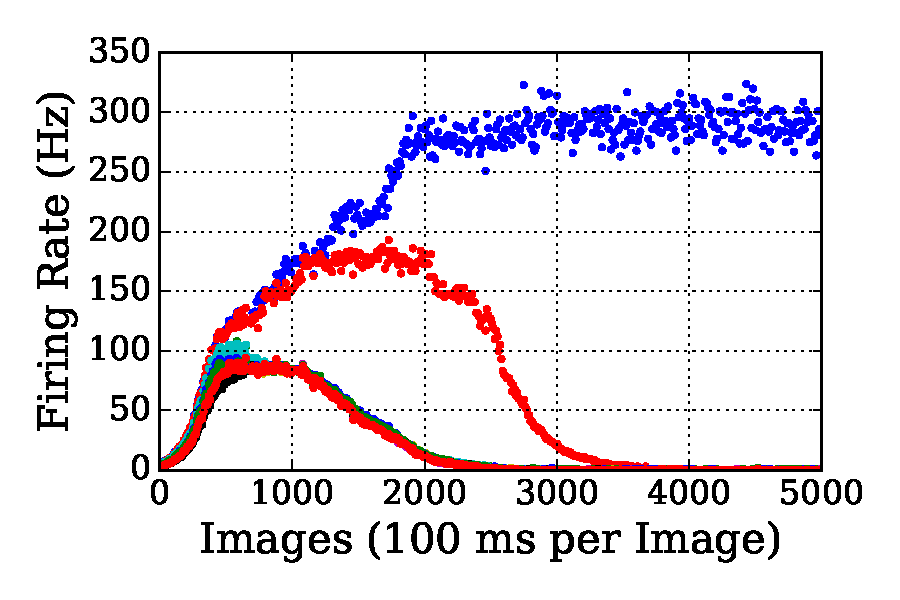
\includegraphics[width=\textwidth]{pics_sdlm/15_exp_SRBM_teach_long/exp1_hid_s.pdf}
		\caption{Output of hidden units in Exp1}
	\end{subfigure}
	\begin{subfigure}[t]{0.45\textwidth}
		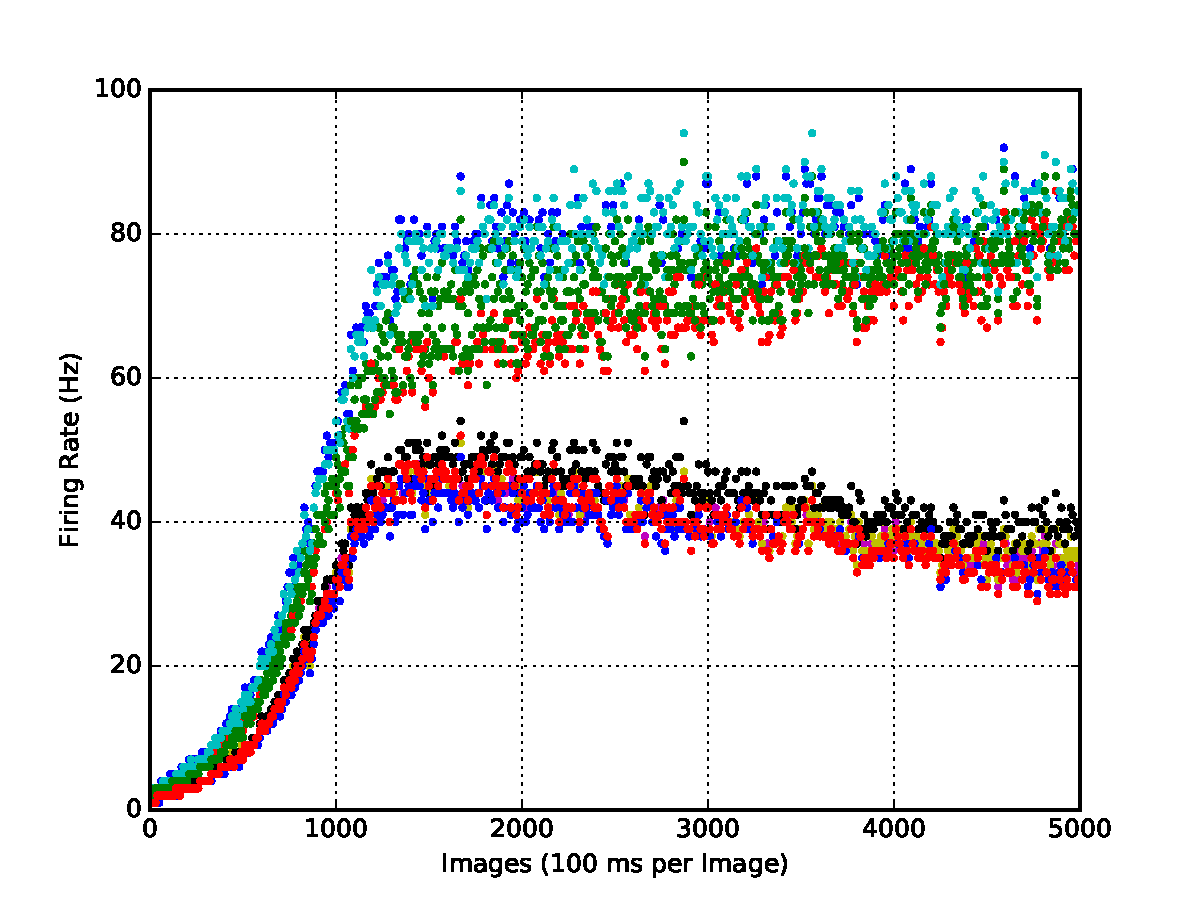
\includegraphics[width=\textwidth]{pics_sdlm/15_exp_SRBM_teach_long/exp2_hid_s.pdf}
		\caption{Output of hidden units in Exp2}
	\end{subfigure}\\
	\begin{subfigure}[t]{0.45\textwidth}
		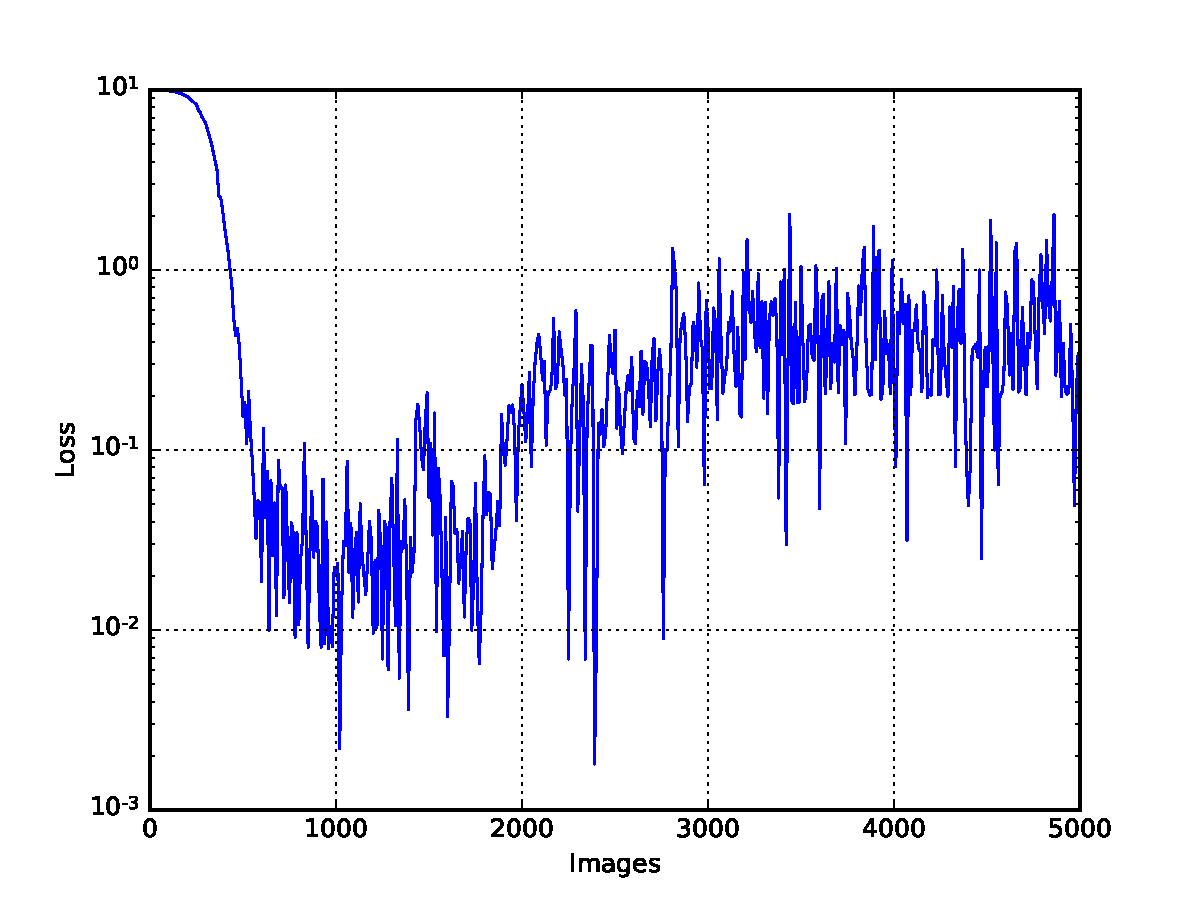
\includegraphics[width=\textwidth]{pics_sdlm/15_exp_SRBM_teach_long/exp1_mse_nons.pdf}
		\caption{Loss of Exp1}
	\end{subfigure}
	\begin{subfigure}[t]{0.45\textwidth}
		\includegraphics[width=\textwidth]{pics_sdlm/15_exp_SRBM_teach_long/exp2_mse_nons.pdf}
		\caption{Loss of Exp2}
	\end{subfigure}
	\caption{Weights and firing rates of visible and hidden units change during training of the reconstruction tests of spiking RBM. 
		Experiments 1) 10 visible units fully connected to 10 hidden units with Poisson spike trains of 100~Hz which lasted 100~ms; 2) same network fed with 10 Poisson spike trains of firing rate ranging from 10~Hz to 100~Hz.}
	\label{fig:sol3_rbm}
\end{figure}

\begin{figure}
	\centering
	\begin{subfigure}[t]{0.45\textwidth}
		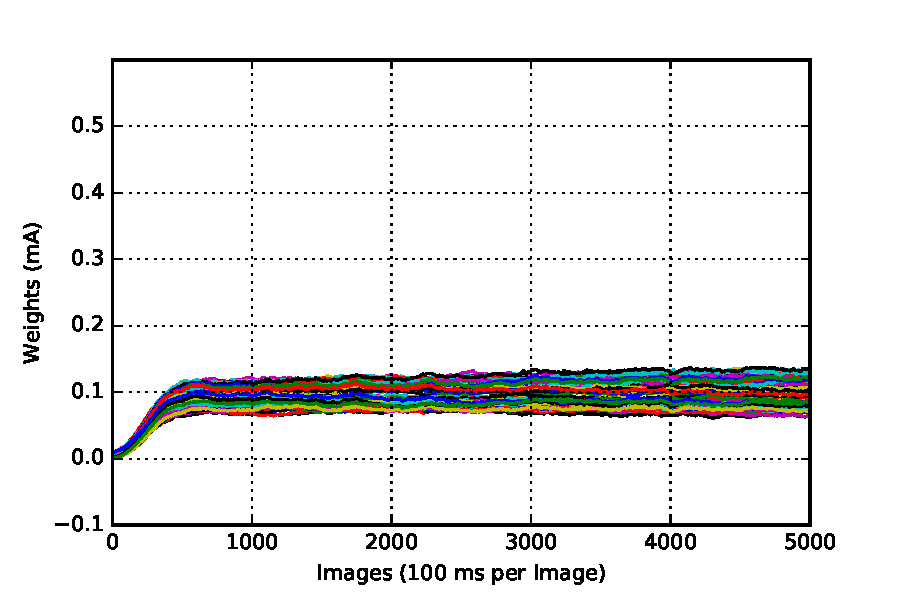
\includegraphics[width=\textwidth]{pics_sdlm/07_exp_SAE_all_long/exp1_weights_s.pdf}
		\caption{Weights of Exp1}
	\end{subfigure}
	\begin{subfigure}[t]{0.45\textwidth}
		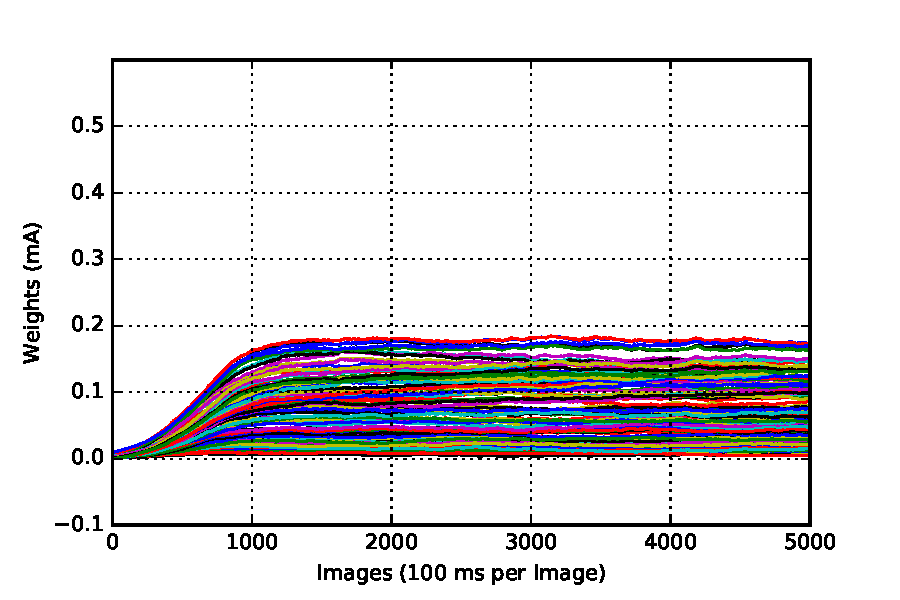
\includegraphics[width=\textwidth]{pics_sdlm/07_exp_SAE_all_long/exp2_weights_s.pdf}
		\caption{Weights of Exp2}
	\end{subfigure}
	\begin{subfigure}[t]{0.45\textwidth}
		\includegraphics[width=\textwidth]{pics_sdlm/07_exp_SAE_all_long/exp1_recon_s.pdf}
		\caption{Reconstruction of visible units in Exp1}
	\end{subfigure}
	\begin{subfigure}[t]{0.45\textwidth}
		\includegraphics[width=\textwidth]{pics_sdlm/07_exp_SAE_all_long/exp2_recon_s.pdf}
		\caption{Reconstruction of visible units in Exp2}
	\end{subfigure}\\
	\begin{subfigure}[t]{0.45\textwidth}
		\includegraphics[width=\textwidth]{pics_sdlm/07_exp_SAE_all_long/exp1_hid_s.pdf}
		\caption{Output of hidden units in Exp1}
	\end{subfigure}
	\begin{subfigure}[t]{0.45\textwidth}
		\includegraphics[width=\textwidth]{pics_sdlm/07_exp_SAE_all_long/exp2_hid_s.pdf}
		\caption{Output of hidden units in Exp2}
	\end{subfigure}\\
	\begin{subfigure}[t]{0.45\textwidth}
		\includegraphics[width=\textwidth]{pics_sdlm/07_exp_SAE_all_long/exp1_mse_nons.pdf}
		\caption{Loss of Exp1}
	\end{subfigure}
	\begin{subfigure}[t]{0.45\textwidth}
		\includegraphics[width=\textwidth]{pics_sdlm/07_exp_SAE_all_long/exp2_mse_nons.pdf}
		\caption{Loss of Exp2}
	\end{subfigure}
	\caption{Weights and firing rates of visible and hidden units change during training of the reconstruction tests of spiking AE. 
		Experiments 1) 10 visible units fully connected to 10 hidden units with Poisson spike trains of 100~Hz which lasted 100~ms; 2) same network fed with 10 Poisson spike trains of firing rate ranging from 10~Hz to 100~Hz.}
	\label{fig:sol4_ae}
\end{figure}

\begin{figure}
	\centering
	\begin{subfigure}[t]{0.45\textwidth}
		\includegraphics[width=\textwidth]{pics_sdlm/17_exp_SRBM_all_long/exp1_weights_s.pdf}
		\caption{Weights of Exp1}
	\end{subfigure}
	\begin{subfigure}[t]{0.45\textwidth}
		\includegraphics[width=\textwidth]{pics_sdlm/17_exp_SRBM_all_long/exp2_weights_s.pdf}
		\caption{Weights of Exp2}
	\end{subfigure}
	\begin{subfigure}[t]{0.45\textwidth}
		\includegraphics[width=\textwidth]{pics_sdlm/17_exp_SRBM_all_long/exp1_recon_s.pdf}
		\caption{Reconstruction of visible units in Exp1}
	\end{subfigure}
	\begin{subfigure}[t]{0.45\textwidth}
		\includegraphics[width=\textwidth]{pics_sdlm/17_exp_SRBM_all_long/exp2_recon_s.pdf}
		\caption{Reconstruction of visible units in Exp2}
	\end{subfigure}\\
	\begin{subfigure}[t]{0.45\textwidth}
		\includegraphics[width=\textwidth]{pics_sdlm/17_exp_SRBM_all_long/exp1_hid_s.pdf}
		\caption{Output of hidden units in Exp1}
	\end{subfigure}
	\begin{subfigure}[t]{0.45\textwidth}
		\includegraphics[width=\textwidth]{pics_sdlm/17_exp_SRBM_all_long/exp2_hid_s.pdf}
		\caption{Output of hidden units in Exp2}
	\end{subfigure}\\
	\begin{subfigure}[t]{0.45\textwidth}
		\includegraphics[width=\textwidth]{pics_sdlm/17_exp_SRBM_all_long/exp1_mse_nons.pdf}
		\caption{Loss of Exp1}
	\end{subfigure}
	\begin{subfigure}[t]{0.45\textwidth}
		\includegraphics[width=\textwidth]{pics_sdlm/17_exp_SRBM_all_long/exp2_mse_nons.pdf}
		\caption{Loss of Exp2}
	\end{subfigure}
	\caption{Weights and firing rates of visible and hidden units change during training of the reconstruction tests of spiking RBM. 
		Experiments 1) 10 visible units fully connected to 10 hidden units with Poisson spike trains of 100~Hz which lasted 100~ms; 2) same network fed with 10 Poisson spike trains of firing rate ranging from 10~Hz to 100~Hz.}
	\label{fig:sol4_rbm}
\end{figure}